\documentclass[12pt]{article}
\usepackage[portuguese]{babel}
\usepackage[utf8]{inputenc}
\usepackage{graphicx}
\usepackage{hyperref}
\usepackage{amsmath}
\usepackage{amssymb}
\usepackage{tikz-cd}
\usepackage{cancel}
\usepackage{hyperref}
\usepackage{xurl}
\usepackage[backend=biber]{biblatex}
\usepackage{eurosym}
\usepackage{multicol}
\usepackage{ragged2e}
\usepackage{csquotes}
\usepackage{listings}
\usepackage{xcolor}
\usepackage{colortbl}
\usepackage{multirow}
\usepackage{indentfirst}
%New colors defined below
\definecolor{codegreen}{rgb}{0,0.6,0}
\definecolor{codegray}{rgb}{0.5,0.5,0.5}
\definecolor{codepurple}{rgb}{0.58,0,0.82}
\definecolor{backcolour}{rgb}{0.95,0.95,0.92}

%Code listing style named "mystyle"
\lstdefinestyle{mystyle}{
  backgroundcolor=\color{backcolour},   commentstyle=\color{codegreen},
  keywordstyle=\color{magenta},
  numberstyle=\tiny\color{codegray},
  stringstyle=\color{codepurple},
  basicstyle=\ttfamily\footnotesize,
  breakatwhitespace=false,         
  breaklines=true,                 
  captionpos=b,                    
  keepspaces=true,                 
  numbers=left,                    
  numbersep=5pt,                  
  showspaces=false,                
  showstringspaces=false,
  showtabs=false,                  
  tabsize=2
}

%"mystyle" code listing set
\lstset{style=mystyle}

\hypersetup{
    colorlinks=true,
    linkcolor=black,  
    urlcolor=blue,
}

\addbibresource{anexos/references.bib}

\makeatletter
\let\latexl@section\l@section
\def\l@section#1#2{\begingroup\let\numberline\@gobble\latexl@section{#1}{#2}\endgroup}
\let\latexl@subsection\l@subsection
\def\l@subsection#1#2{\begingroup\let\numberline\@gobble\latexl@subsection{#1}{#2}\endgroup}
\let\latexl@subsubsection\l@subsubsection
\def\l@subsubsection#1#2{\begingroup\let\numberline\@gobble\latexl@subsubsection{#1}{#2}\endgroup}
\renewcommand{\@seccntformat}[1]{}
\makeatother
\usepackage[hmargin=3.05cm,vmargin=3.5cm,bmargin=2cm]{geometry}

\begin{document}

    \begin{center}
        \vspace*{1cm}
            
        \Huge
        \textbf{Trabalho Prático}
        
        \vspace{0.5cm}
        \textbf{Matemática Discreta}     
        
        \vspace{1.5cm}
        \Large{Autores: \\
        Bruno Dylan Pinto Ferreira 8200586\\
        Gonçalo André Fontes Oliveira 8200595 \\ 
        Jorge Miguel Fernandes Correia 8200592\\
        Nuno de Figueiredo Brito e Castro 8200591}
        
        \vspace{0.5cm}
        \Large{Grupo: 17}
        
        \vspace{0.5cm}
         \Large{Licenciatura em Engenharia Informática \\ 2020/2021}
          \vspace{1.5cm}
         \begin{figure}[h!]\centering
            
\includegraphics[scale=0.4]{anexos/logo_estg.png}
        \end{figure}
         
        \thispagestyle{empty}
    \end{center}
    
    \newpage
    \renewcommand{\contentsname}{Índice}
    \tableofcontents
    \newpage
    \section{Introdução}
    
     \noindent No âmbito da unidade curricular de matemática discreta foi-nos proposta a resolução de 3 questões relacionadas com a matéria lecionada ao longo do 2º semestre como:

    \begin{itemize}
    \item Indução Matemática ou aplicação do algoritmo EGV( Expand, Guess, Verify):
    O Método de Indução Matemática é um método que tem por base o Princípio de Indução Finita que é bastante utilizado para comprovar se determinadas propriedades são verdadeiras tendo em conta o conjunto dos números naturais.
    \item Teoria dos grafos é um ramo da matemática que estuda as relações entre os objetos de um determinado conjunto. Para tal são empregadas estruturas chamadas de grafos, G(V,E), onde V é um conjunto não vazio de objetos denominados vértices e E é um subconjunto de pares não ordenados de V denominados de arestas.
    \item Em criptografia, \textbf{encriptação} é o processo de transformar informação usando um algoritmo, chamado de cifra, de modo a impossibilitar a sua leitura. Por isso, ao processo de tornar informação encriptada novamente legível dá-se o nome de \textbf{desencriptação}.

    \end{itemize}
    
    \noindent Este relatório está estruturado em 3 partes onde damos solução aos diversos exercícios propostos no enunciado explicando toda a resolução realizada até ao resultado final.
    \\\\Começamos por resolver um exercício que aborda a aplicação do método EGV onde começamos por apresentar a nossa função e os respetivos passos dados até à sua resolução final. Em cada passo além dos cálculos pode ser visualizada uma breve explicação do que foi realizado o que torna mais fácil a perceção do que foi feito no exercício.\\
    
    \noindent Seguidamente resolvemos um exercício referente à matéria de Teoria dos Grafos. Neste exercício aplicamos diversos conhecimentos desta matéria que fomos obtendo ao longo do semestre. O exercício envolve monumentos e alojamentos da Rota do Românico e consiste em calcularmos caminhos e/ou circuitos obedecendo a determinadas condições e utilizando diferentes algoritmos.\\
    
    \noindent Por fim, resolvemos um exercício que diz respeito à matéria de Criptografia que está subdividido em duas partes: Encriptação e Desencriptação. Neste exercício necessitamos de completar uma frase que depois é encriptada utilizando algoritmos. Após a encriptação dessa mensagem é necessário desencriptá-la para que esta volte a ser legível.
     
    \newpage
    \noindent\textbf{Nota:} Ao longo da realização deste trabalho prático tivemos o cuidado de apresentar o uso de um algoritmo através de cálculos realizados por nós e através do uso de um algoritmo feito em Python, desenvolvido também por nós. O uso da linguagem Python para desenvolver um algoritmo que fosse capaz de resolver o exercício foi uma forma muito mais fácil e eficaz sendo que nos poupa bastante trabalho e tempo em cálculos e, além disso a taxa de erro na resolução dos cálculos é muito menor.\\
    
     \noindent Com a realização deste trabalho vamos aprofundar os conceitos lecionados durante o 2º semestre na unidade curricular de Matemática Discreta. Estes conceitos serão importantes para o nosso futuro dado que podem ser vir a utilizados no desenvolvimento de futuros projetos.   
    
    \newpage
    
    \section{Resolução dos exercícios}
    
    \subsection{1. Exercício EGV}
   \noindent \textbf{Nesta questão é proposto fazer a aplicação do algoritmo EGV(Expand, Guess, Verify = Desenvolver, Estimar, Verificar) que consiste em encontrar a sua fórmula fechada.}\\

   
   
     \[
        \begin{cases} 
          f(1) = 2  \\ 
          f(n) = 2 \times f(n - 1) + 2^n \mbox{ para }  n\geqslant 2 
       \end{cases}
    \]
    \vspace{0.5cm}
    \\
   
    \noindent \textbf{Expand} - Este passo consiste em utilizar a fórmula de recorrência da função 
apresentada e expandi-la da seguinte forma:  \\
Começar por \(f(n)\), que é função de \(f(n - 1)\):\\
Calcular \(f(n-1)\) e substituir em \(f(n)\), obtendo-se assim \(f(n)\) em função de
\(f(n - 2)\).\\
Calcular \(f(n - 2)\) e substituir em \(f(n)\), obtendo-se assim \(f(n)\) em função de
\(f(n - 3)\).\\
Calcular \(f(n - 3)\) e substituir em \(f(n)\), obtendo-se assim \(f(n)\) em função de
\(f(n - 4)\).\\
 \\
 Tendo isto em conta obtemos que: 
    \\
    \(f(n) = 2 \times f(n - 1) + 2^n \)\\
    \(\hspace*{0.9cm}= 2 \times (2 \times f(n - 2) + 2^{n-1} )+ 2^n = 2^2 \times f(n - 2) + 2^{n} + 2^n = 2^2 \times f(n - 2) + 2 \times 2^n\)\\
    \(\hspace*{0.9cm}= 2^2(2 \times f(n - 3) + 2^{n-2})+ 2 \times 2^n = 2^3 \times f(n - 3) + 3 \times 2^n\)\\
    \(\hspace*{0.9cm}= 2^3 (2 \times f(n - 4) + 2^{n-3}) + 3 \times  2^n = 2^4 \times f(n - 4) + 4 \times 2^n\)\\
    
    \noindent \textbf{Guess} -  
    Neste passo utilizou-se a fórmula final obtida através do passo Expand para mostrar qual é a nossa definição, onde \( k \) representa o nosso argumento. Em seguida consideramos que \(n - k = 1 \) logo \( k = n - 1\)\\
    Então, podemos conjeturar que: \\\\
    \(f(n) = 2^k \times f(n - k) + k \times 2^{n}\)\\\\
    Se \(n - k = 1 (=) k = n - 1\), temos \\\\
    \(f(n) = 2^{n-1} \times f(n - (n - 1)) + (n-1) \times 2^{n}\)\\
    \(\hspace*{0.9cm}= 2^{n-1} \times f(1)  + (n-1) \times 2^{n}\)\\
    \(\hspace*{0.9cm}= 2^{n-1} \times 2  + n\times2^{n} - 2^{n}\)\\
    \(\hspace*{0.9cm}= 2^{n}  + n\times2^{n} - 2^{n}\)\\
    \(\hspace*{0.9cm}= n\times2^{n}\)\\
    \newpage
    \noindent \textbf{Verify} - Por fim podemos verificar que a nossa fórmula fechada está correta através de uma demonstração indutiva, que se divide em dois passos:\\\\
    \textbf{Passo Base} - Neste passo pretendemos mostrar que a fórmula se verifica para n = 1, sendo 1 um valor inicial. Por isso, fazendo os respetivos cálculos podemos observar que os valores se confirmam:\newline\newline\hspace*{4cm}\(f(1)= 1\times2^{1}=2\) \textbf{\textcolor{codegreen}{Verdadeiro}}\newline \\
    \textbf{Passo indutivo (Hipótese)} - Neste passo temos de mostrar que se a fórmula se confirma para n = k,
    então a mesma fórmula confirma-se para n = k + 1, ou seja, provando assim que o processo usado na passagem de um valor para o valor seguinte é válido. Supondo que a expressão n = k é verdadeira, substitui-se os n's por k e assim apresentamos a nossa Hipótese: \newline\newline\hspace*{4cm}\(f(k)= k\times2^{k}\)\newline\\
    \textbf{Passo indutivo (Tese)} - De seguida é necessário provar a que a nossa tese é válida, começando por igualar \(f(k+1)\) à fórmula de recorrência com as respetivas substituições de n por k + 1.\\
    \newline
    
    \begin{center}
        \begin{tabular}{@{}l@{}}
            \(f(k+1) = 2\times f(k+1-1) + 2^{k+1} = 2 \times f(k) + 2^{k+1}\), por definição de f \\
            \hspace*{1.65cm}\(= 2\times k \times 2^{k} \times 2^{k+1}\), pela hipótese de indução \\
            \hspace*{1.65cm}\(= k \times 2^{k+1} \times 2^{k+1} = (k+1) \times 2^{k+1}\), c.q.m \\
        \end{tabular}
    \end{center}
    \newpage
    
    \subsection{2. Exercício Teoria dos grafos}
    
    
    \noindent Neste exercício é proposto que criemos um grafo com 6 vértices em que 5 representam monumentos da Rota do Românico e o 6º representa o alojamento para pernoitar que deve estar localizado dentro da região da Rota do Românico.Decidimos criar um percurso no qual os nossos visitantes desfrutem dos seguintes locais Ponto do arco, Memorial da Ermida, Igreja de Santa Maria de Airães, Centro de Interpretação do românico, Igreja de São Pedro de Abragão e tivemos em conta número de kms percorridos, consumo de combustível (gasóleo com o custo de 1,283\euro por litro) e portagens (caso existam).
    \newline \newline
    \noindent Para a elaboração do exercício foram usadas abreviaturas para definir os pontos e também foram levados em consideração 3 critérios:
    
    \begin{enumerate}
    \item  Abreviaturas:
        \begin{itemize}
        \item   Casas do Telhado (Penafiel) - CT;
        \item   Ponto do arco (Marco Canaveses) - PA;
        \item   Memorial da Ermida (Penafiel) - ME;
        \item   Igreja de Santa Maria de Airães (Felgueiras) - ISMA;
        \item   Centro de Interpretação do românico (Lousada) - CI;
        \item   Igreja de São Pedro de Abragão (Penafiel) - ISPA;
        \item   Interseções- IN.        
    \end{itemize}
    \item  Critérios:
        \begin{itemize}
        \item   Número de kms percorridos;
        \item   Consumo de combustível e portagens (caso existam);
        \item   Tempo despendido na viagem.
        \end{itemize}
    \end{enumerate}
    
    \newpage
    
    \subsubsection{Representação real do Grafo}
    \noindent É possível aceder a esta representação pelo link seguinte: 
    \url{https://www.google.com/maps/d/u/0/edit?mid=1gjb0kchVgrH6ip_8DapSzaq5lc3uEJs0&usp=sharing}
    \\
    \begin{center}
    
        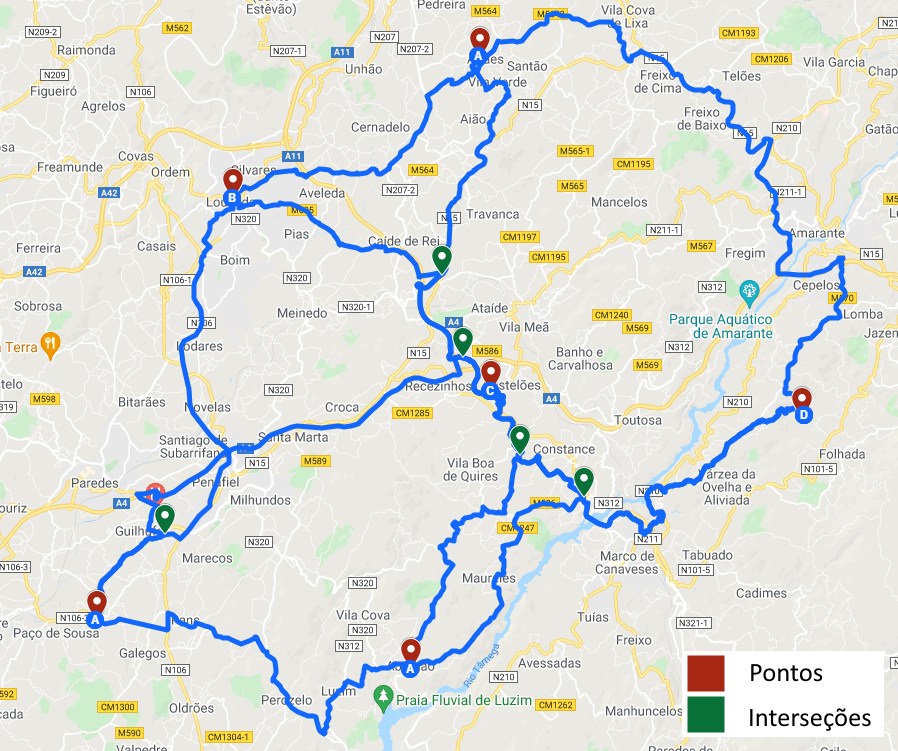
\includegraphics[scale=0.65]{anexos/mapa.png}
    \end{center}
        
    \newpage
    
    
    \subsubsection{Representação do Grafo}
    \noindent Para resolver o problema acima foi então criado um novo vértice  (Inter) como podemos ver abaixo
    
    \begin{center}
        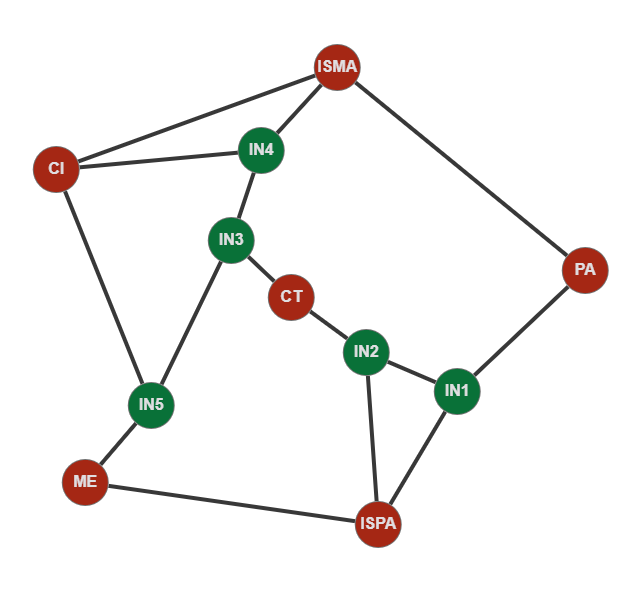
\includegraphics[scale=0.7]{anexos/grafoV1.png}
    \end{center}
    
    \begin{itemize}
    \item \noindent V(G) = \{ISMA, CT, PA, ISPA, ME, CI, IN1, IN2, IN3, IN5, IN4\} 
    \item \noindent E(G) = \{(ISMA, CI), (ISMA, IN4), (ISMA, PA), (CI, IN4), (CI, IN5), (IN4, IN3), (PA, IN1),(IN5, ME), (IN5, IN3), (IN3, CT), (IN1, IN2), (IN1, ISPA), (ME, ISPA), (CT, IN2), (IN2, ISPA)\}
    \item Ordem do Grafo - 11 vértices
    \item Dimensão do Grafo - 15 arestas
    \end{itemize}
    
    \newpage
    
    \begin{tabular}{@{}m{\dimexpr.5\textwidth-.5\columnsep}m{\dimexpr.5\textwidth-.5\columnsep}@{}}
       \begin{center}
           \noindent \textbf{Matriz de adjacência}\\
       \end{center}
    
        \noindent
        $$
        \left[
            \begin{array}{*{11}c}
                0 & 0 & 1 & 0 & 0 & 1 & 0 & 0 & 0 & 0 & 1\\ 
                0 & 0 & 0 & 0 & 0 & 0 & 0 & 1 & 1 & 0 & 0\\ 
                1 & 0 & 0 & 0 & 0 & 0 & 1 & 0 & 0 & 0 & 0\\ 
                0 & 0 & 0 & 0 & 1 & 0 & 1 & 1 & 0 & 0 & 0\\ 
                0 & 0 & 0 & 1 & 0 & 0 & 0 & 0 & 0 & 1 & 0\\ 
                1 & 0 & 0 & 0 & 0 & 0 & 0 & 0 & 0 & 1 & 1\\ 
                0 & 0 & 1 & 1 & 0 & 0 & 0 & 1 & 0 & 0 & 0\\ 
                0 & 1 & 0 & 1 & 0 & 0 & 1 & 0 & 0 & 0 & 0\\ 
                0 & 1 & 0 & 0 & 0 & 0 & 0 & 0 & 0 & 1 & 1\\ 
                0 & 0 & 0 & 0 & 1 & 1 & 0 & 0 & 1 & 0 & 0\\ 
                1 & 0 & 0 & 0 & 0 & 1 & 0 & 0 & 1 & 0 & 0 
            \end{array}
            \right]
        $$ 
      &
        \vspace*{1.5cm}
        \noindent Grau(ISMA) = 3 \newline
        \noindent Grau(CT) = 2 \newline
        \noindent Grau(PA) = 2 \newline
        \noindent Grau(ISPA) = 3 \newline
        \noindent Grau(ME) = 2 \newline
        \noindent Grau(CI) = 3 \newline
        \noindent Grau(IN1) = 3 \newline
        \noindent Grau(IN2) = 3 \newline
        \noindent Grau(IN3) = 3 \newline
        \noindent Grau(IN5) = 3 \newline
        \noindent Grau(IN4) = 3 \newline
    \end{tabular}
    
    \noindent Ordem dos vértices: ISMA, CT, PA, ISPA, ME, CI, IN1, IN2, IN3, IN5, IN4\\
    
    \subsubsection{Classificação do grafo}
    
    \begin{enumerate}
      \item Grafo Simples.
        \begin{itemize}
          \item O grafo é simples porque cada aresta liga dois vértices diferentes,
                nenhuma aresta liga um vértice a si mesmo e
                não existem duas arestas diferentes que ligam os mesmos vértices.
        \end{itemize}
      
      \item Grafo não orientado
          \begin{itemize}
              \item O grafo é não orientado porque as arestas não possuem direções, por isso a matriz de adjacências é simétrica\\
              
            $$
            \left[
                \begin{array}{*{11}c}
                    0 & 0 & 1 & 0 & 0 & 1 & 0 & 0 & 0 & 0 & 1\\ 
                    0 & 0 & 0 & 0 & 0 & 0 & 0 & 1 & 1 & 0 & 0\\ 
                    1 & 0 & 0 & 0 & 0 & 0 & 1 & 0 & 0 & 0 & 0\\ 
                    0 & 0 & 0 & 0 & 1 & 0 & 1 & 1 & 0 & 0 & 0\\ 
                    0 & 0 & 0 & 1 & 0 & 0 & 0 & 0 & 0 & 1 & 0\\ 
                    1 & 0 & 0 & 0 & 0 & 0 & 0 & 0 & 0 & 1 & 1\\ 
                    0 & 0 & 1 & 1 & 0 & 0 & 0 & 1 & 0 & 0 & 0\\ 
                    0 & 1 & 0 & 1 & 0 & 0 & 1 & 0 & 0 & 0 & 0\\ 
                    0 & 1 & 0 & 0 & 0 & 0 & 0 & 0 & 0 & 1 & 1\\ 
                    0 & 0 & 0 & 0 & 1 & 1 & 0 & 0 & 1 & 0 & 0\\ 
                    1 & 0 & 0 & 0 & 0 & 1 & 0 & 0 & 1 & 0 & 0 
                \end{array}
                \right]
            $$ 
            \end{itemize}
    Ordem dos vértices: ISMA, CT, PA, ISPA, ME, CI, IN1, IN2, IN3, IN5, IN4\\
            
    \item Grafo Semi-Hamiltoniano
        \begin{itemize}
              \item O grafo semi-Hamiltoniano é um grafo que admite um caminho de Hamilton.
              \begin{itemize}
              \item Um caminho de Hamilton é um caminho num grafo que passa em cada vértice
exatamente uma vez.

              \end{itemize}
            
                       

            \item \textbf{Exemplo de um caminho de hamilton do grafo}: (ISMA, PA, IN1, ISPA, ME, IN5, CI, IN4, IN3, CT, IN2)
            
            \centering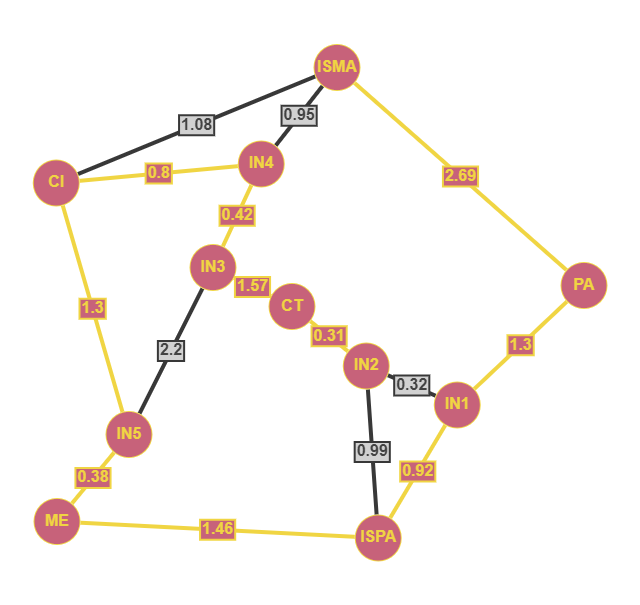
\includegraphics[scale=0.4]{anexos/caminho_hamilton.png} 
            \end{itemize}
            
        \item Grafo conexo e fortemente conexo
            \begin{itemize}
              \item Um grafo não orientado diz-se conexo se, para cada par de vértices, existe um
                    caminho que os une. Caso contrário, o grafo diz-se desconexo.
               \item Pode-se dizer também que um grafo não orientado é conexo (fortemente conexo) se o fecho transitivo da sua matriz de adjacências não tiver entradas nulas.
               \item O fecho transitivo de uma matriz de adjacências M, de ordem n, de um grafo G é a matriz F definida por: \newline\break $ F = M + M^{2} + M^{3} + M^{4} + M^{5} + M^{6} + M^{7} + M^{8} + M^{9} + M^{10} + M^{11} $ 
            
             \scalebox{0.8}{
            $
                =\left[
                \begin{array}{*{11}c}
                    16647 & 9197 &  10009 & 10722 & 9197 &  18353 & 10695 & 10722 & 15430 & 15430 & 18353\\
                9197 &  5459 &  6352 &  7849 &  7011 &  10824 & 8381 &  9016 &  10173 & 7649 &  8976\\ 
                10009 & 6352 &  6398 &  8287 &  6352 &  10472 & 8615 &  8287 &  9291 &  9291 &  10472\\
                10722 & 7849 &  8287 &  12016 & 9016 &  11842 & 12532 & 12887 & 11521 & 9673 &  10485\\
                9197 &  7011 &  6352 &  9016 &  5459 &  8976 &  8381 &  7849 &  7649 &  10173 & 10824\\
                18353 & 10824 & 10472 & 11842 & 8976 &  18865 & 11419 & 10485 & 15337 & 18352 & 21093\\
                10695 & 8381 &  8615 &  12532 & 8381 &  11419 & 12277 & 12532 & 10685 & 10685 & 11419\\
                10722 & 9016 &  8287 &  12887 & 7849 &  10485 & 12532 & 12016 & 9673 &  11521 & 11842\\
                15430 & 10173 & 9291 &  11521 & 7649 &  15337 & 10685 & 9673 &  12411 & 16487 & 18352\\
                15430 & 7649 &  9291 &  9673 &  10173 & 18352 & 10685 & 11521 & 16487 & 12411 & 15337\\
                18353 & 8976 &  10472 & 10485 & 10824 & 21093 & 11419 & 11842 & 18352 & 15337 & 18865 
                \end{array}
                \right]
             $}
               
                \item Podemos concluir assim que o grafo é conexo e fortemente conexo, pois se grafo não orientado é conexo logo é também fortemente conexo.
            \end{itemize}
        
    \end{enumerate}
    
    \noindent\textbf{Nota:} O grafo não é euleriano ou semi-euleriano porque não admite um circuito ou caminho de Euler, respetivamente. Além disso os graus não são todos pares nem existem apenas 2 graus ímpares.\\\\
    
    \newpage
    
    \subsubsection{Tabela dos critérios para o custo}
    \noindent Nesta tabela encontram-se todos os caminhos que ligam os diferentes vértices e, o seu respetivo custo para que fosse mais fácil identificar o mais "rentável". Para estes cálculos usamos a os dados fornecidos pela a aplicação Waze.\newline
    
    \noindent Para este exercício consideramos que um automóvel gasta 1 litro de gasóleo a cada 12 Km. Dado que o preço do gasóleo no  momento se encontra a 1,283\euro \hspace{1mm}por litro, o preço do gasóleo por Km é \( \frac{1,283}{12}\).\\\\
    \begin{center}
        Km \(\times \hspace{1mm} \frac{1,283}{12}\) + portagens\\
    \end{center} 
    
    \begin{table}[hbt!]
        \scalebox{0.73}{
    \begin{tabular}{|c|c|c|c|c|c|c|}
    \hline
    \textbf{Vértice 1} & \textbf{Vértice 2} & \textbf{km} & \textbf{Tempo viagem} & \textbf{Preço gasóleo gasta} & \textbf{Preço portagens} & \textbf{Total preço} \\ \hline
    PA                 & ISMA               & 25,2 km     & 35 min                & 2,69\euro                        & Sem portagem                 & 2,69\euro   \\ \hline
    PA                 & IN1                & 12,2 km     & 21 min                & 1,30\euro                        & Sem portagem                 & 1,30\euro   \\ \hline
    ME                 & ISPA               & 13,7 km     & 22 min                & 1,46\euro                        & Sem portagem                 & 1,46\euro   \\ \hline
    ME                 & IN5                & 3,6 km      & 6 min                 & 0,38\euro                        & Sem portagem                 & 0,38\euro   \\ \hline
    ISMA               & CI                 & 10,1 km     & 18 min                & 1,08\euro                         & Sem portagem                 & 1,08\euro   \\ \hline
    ISMA               & IN4                & 8,8 km      & 14 min                & 0,95\euro                         & Sem portagem                 & 0,95\euro   \\ \hline
    CI                 & IN4                & 7,5 km      & 13 min                & 0,80\euro                         & Sem portagem                 & 0,80\euro    \\ \hline 
    CI                 & IN5                & 12,2 km     & 19 min                & 1,30\euro                        & Sem portagem                 & 1,30\euro   \\ \hline
    ISPA               & IN1                & 8,6 km      & 18 min                & 0,92\euro                        & Sem portagem                 & 0,92\euro   \\ \hline
    ISPA               & IN2                & 9,3 km      & 23 min                & 0,99\euro                        & Sem portagem                 & 0,99\euro   \\ \hline
    CT                 & IN3                & 10 km       & 9 min                 & 1,07\euro                        & 0,50                         & 1,57\euro   \\ \hline
    CT                 & IN2                & 2,9 km      & 5 min                 & 0,31\euro                         & Sem portagem                 & 0,31\euro    \\ \hline
    IN1                & IN2                & 3 km        & 5 min                 & 0,32\euro                         & Sem portagem                 & 0,32\euro    \\ \hline 
    IN3                & IN4                & 3,9 km      & 3 min                 & 0,42\euro                            & 0,25                         & 0,42\euro    \\ \hline
    IN3                & IN5                & 20,6 km     & 16 min                & 2,20\euro                        & 1,35                         & 2,20\euro   \\ \hline

    \end{tabular}}
    \end{table}
    
    \newpage
    
    \subsubsection{Representação do Grafo com custos}
    \noindent Neste grafo foram adicionados os custos
    
    \begin{center}
        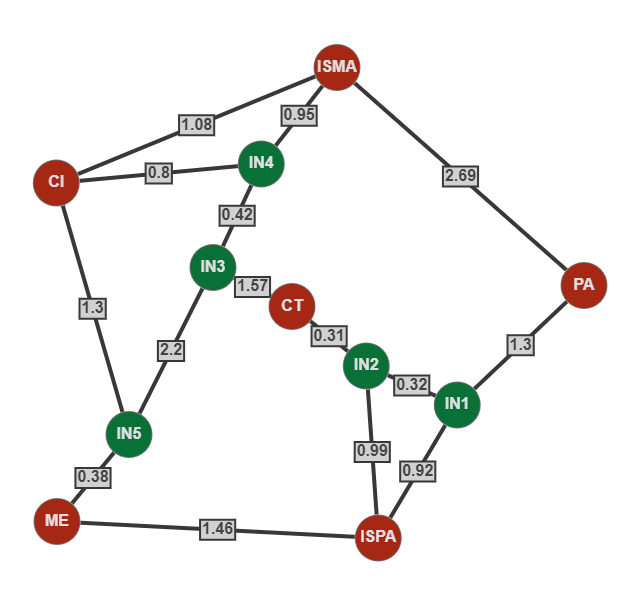
\includegraphics[scale=0.7]{anexos/grafo_custos.png}
    \end{center}
    
    \begin{center}
        \noindent \textbf{Matriz de custos}
    \end{center}
    
    $$
        \left[
            \begin{array}{*{11}c}
               			0 & \infty& 2,69 & \infty& \infty& 1,08 & \infty& \infty& \infty& \infty& 0,95 \\ 
                \infty& 0 & \infty& \infty& \infty& \infty& \infty& 0,31 & 1,57 & \infty& \infty\\ 
                2,69 & \infty& 0 & \infty& \infty& \infty& 1,3 & \infty& \infty& \infty& \infty\\ 
                \infty& \infty& \infty& 0 & 1,46 & \infty& 0,92 & 0,99 & \infty& \infty& \infty\\ 
                \infty& \infty& \infty& 1,46 & 0 & \infty& \infty& \infty& \infty& 0,38 & \infty\\ 
                1,08 & \infty& \infty& \infty& \infty& 0 & \infty& \infty& \infty& 1,3 & 0,8 \\ 
                \infty& \infty& 1,3 & 0,92 & \infty& \infty& 0 & 0,32 & \infty& \infty& \infty\\ 
                \infty& 0,31 & \infty& 0,99 & \infty& \infty& 0,32 & 0 & \infty& \infty& \infty\\ 
                \infty& 1,57 & \infty& \infty& \infty& \infty& \infty& \infty& 0 & 2,2 & 0,42 \\ 
                \infty& \infty& \infty& \infty& 0,38 & 1,3 & \infty& \infty& 2,2 & 0 & \infty\\ 
                0,95 & \infty& \infty& \infty& \infty& 0,8 & \infty& \infty& 0,42 & \infty& 0
            \end{array}
            \right]
    $$
    
    \noindent Ordem dos vértices: ISMA, CT, PA, ISPA, ME, CI, IN1, IN2, IN3, IN5, IN4\\
    
    \newpage
    \subsubsection{a) O percurso com menor custo com origem no alojamento e destino no monumento mais distante dos 5 escolhidos (não necessariamente passando por todos)}

    
        \begin{table}[hbt!]
            \centering
            \begin{tabular}{*{4}{|c}|}
            \hline
            \textbf{Vértice 1} & \textbf{Vértice 2} & \textbf{Caminho} & \textbf{Km}\\ \hline
            CT                & ISMA     & (CT,IN3,IN4,ISMA)          & 22,7 Km     \\ \hline
            CT                 & PA      & (CT,IN2,IN1,PA)          & 18,1 Km     \\ \hline
            CT                 & ISPA    & (CT,IN2,ISPA)           & 12,2 Km     \\ \hline
            \rowcolor{codegreen} \textcolor{white}{\textbf{CT}}                 & \textcolor{white}{\textbf{ME}}      & \textcolor{white}{\textbf{(CT,IN3,IN5,ME)}}          & \textcolor{white}{\textbf{34.2 Km}}     \\ \hline
            CT               & CI        & (CT,IN3,IN4,CI)         & 21,4 Km     \\ \hline
        
            \end{tabular}
        \end{table}
        \noindent Como é possível visualizar na tabela acima, o monumento com maior distância do local de alojamento é o Memorial da Ermida (ME) com 34.2 Km.\\
        
        \noindent Após obtido o monumento mais distante do alojamento, é pedido para encontrar o percurso com menor custo com origem no alojamento e destino no monumento ME (Memorial da Ermida). Para isso utilizamos o algoritmo de Dijkstra:\\
        
        \noindent O algoritmo de Dijkstra, concebido pelo cientista da computação holandês Edsger Dijkstra em 1956 e publicado em 1959, soluciona o problema do caminho mais curto num grafo orientado ou não orientado com arestas de peso não negativo, em tempo computacional onde V é o número de vértices e E é o número de arestas.\\
        
        \begin{table}[hbt!]
            \centering
            \scalebox{0.7}{
            \begin{tabular}{*{9}{|c}|}
            \hline
            \textbf{ } & \textbf{Passo 1} & \textbf{Passo 2} & \textbf{Passo 3} & \textbf{Passo 4} & \textbf{Passo 5} & \textbf{Passo 6} & \textbf{Passo 7} & \textbf{Passo 8}\\ \hline
             CT & {\cellcolor{codegreen}\textcolor{white}{\textbf{(O, CT)}}} & $\infty$ & $\infty$ & $\infty$ & $\infty$ & $\infty$ & $\infty$ & $\infty$ \\ \hline
             IN3 & (1.57, CT) & (1.57, CT) & (1.57, CT) & (1.57, CT) & {\cellcolor{codegreen}\textcolor{white}{\textbf{(1.57, CT)}}} & $\infty$ & $\infty$ & $\infty$ \\ \hline
             IN4 & $\infty$ & $\infty$ & $\infty$ & $\infty$ & $\infty$ & (1.99, IN3) & {\cellcolor{codegreen}\textcolor{white}{\textbf{(1.99, IN3)}}} & $\infty$ \\ \hline
             ISMA & $\infty$ & $\infty$ & $\infty$ & $\infty$ & $\infty$ & $\infty$ & (4.62, PA) & (2.94, IN4) \\ \hline
             PA & $\infty$ & $\infty$ & $\infty$ & (1.93, IN1) & (1.93, IN1) & {\cellcolor{codegreen}\textcolor{white}{\textbf{(1.93, IN1)}}} & $\infty$ & $\infty$ \\ \hline
             IN1 & $\infty$ & (0.63, IN2) & {\cellcolor{codegreen}\textcolor{white}{\textbf{(0.63, IN2)}}} & $\infty$ & $\infty$ & $\infty$ & $\infty$ & $\infty$ \\ \hline
             IN2 & (0.31, CT) & {\cellcolor{codegreen}\textcolor{white}{\textbf{(0.31, CT)}}} & $\infty$ & $\infty$ & $\infty$ & $\infty$ & $\infty$ & $\infty$ \\ \hline
             \multirow{2}*{ISPA} & $\infty$ & (1.3, IN2) & (1.3, IN2) & {\cellcolor{codegreen}\textcolor{white}{\textbf{\textcolor{red}{\xcancel{(1.55, IN1)}}}}} & $\infty$ & $\infty$ & $\infty$ & $\infty$ \\
             &  &  &  & {\cellcolor{codegreen}\textcolor{white}{(1.3, IN2)}} &  &  &  &  \\\hline
             ME & $\infty$ & $\infty$ & $\infty$ & $\infty$ & (2.76, ISPA) & (2.76, ISPA) & (2.76, ISPA) & {\cellcolor{codegreen}\textcolor{white}{\textbf{(2.76, ISPA)}}} \\ \hline
             IN5 & $\infty$ & $\infty$ & $\infty$ & $\infty$ & $\infty$ & (3.77, IN3) & (3.77, IN3) & (3.77, IN3) \\ \hline
             CI & $\infty$ & $\infty$ & $\infty$ & $\infty$ & $\infty$ & $\infty$ & $\infty$ & (2.79, IN4) \\ \hline
            \end{tabular}}
        \end{table}
        
    \noindent Caminho de menor custo de CT para ME :  
   \begin{enumerate}
       \item Fazer o caminho de ME para CT : ME, ISPA, IN2, CT
       \item Colocar o caminho do ultimo vértice para o primeiro vértice: CT, IN2, ISPA, ME
   \end{enumerate}
   \newpage
    \subsubsection{b) O percurso com menor custo entre cada dois locais}
    \noindent Para tornar o processo do algoritmo de Dijkstra, mais fácil e rápido decidimos criar um programa em Python.\\\\
    Este programa recebe o número de vértices, os nomes dos vértices, os seus pesos (como o nosso grafo é não orientado apenas é lida a diagonal inferior), por fim é pedido o vértice inicial e o vértice final. Para criar o programa utilizamos a seguinte biblioteca \url{https://gitlab.com/AlanDeSmet/dijkstra-spf/-/tree/master}  que nos dá o caminho de Dijkstra num gráfico não orientado.\\
    
   \noindent  \textbf{Casas do telhado para Ponto do arco:}\\
    \begin{tabular}{@{}m{\dimexpr.5\textwidth-.5\columnsep}m{\dimexpr.5\textwidth-.5\columnsep}@{}}
      \centering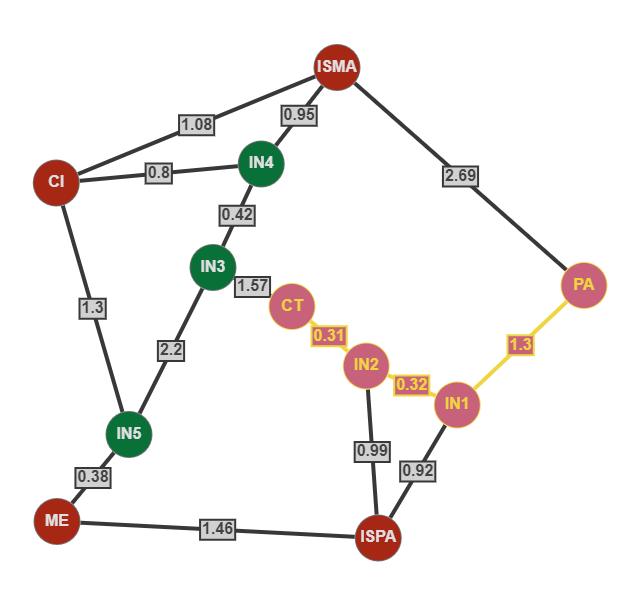
\includegraphics[scale=0.4]{anexos/CT-PA.png} &
      \begin{itemize}
        \item  Percurso: CT $\rightarrow$ IN2 $\rightarrow$ IN1 $\rightarrow$ PA
        \item  Custo final: 1,93
      \end{itemize}
    \end{tabular}
    
    \noindent \textbf{Casas do telhado para Memorial da Ermida:}\\
    \begin{tabular}{@{}m{\dimexpr.5\textwidth-.5\columnsep}m{\dimexpr.5\textwidth-.5\columnsep}@{}}
      \centering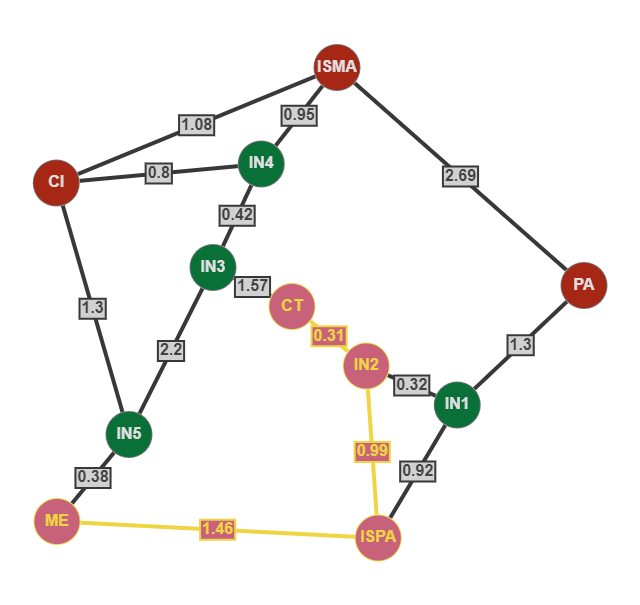
\includegraphics[scale=0.4]{anexos/CT-ME.png} &
      \begin{itemize}
        \item  Percurso: CT $\rightarrow$ IN2 $\rightarrow$ ISPA $\rightarrow$ ME
        \item  Custo final: 2,76
      \end{itemize}
    \end{tabular}
    \newpage
   \noindent\textbf{ Casas do telhado para Igreja de Santa Maria de Airães:}\\
    \begin{tabular}{@{}m{\dimexpr.5\textwidth-.5\columnsep}m{\dimexpr.5\textwidth-.5\columnsep}@{}}
      \centering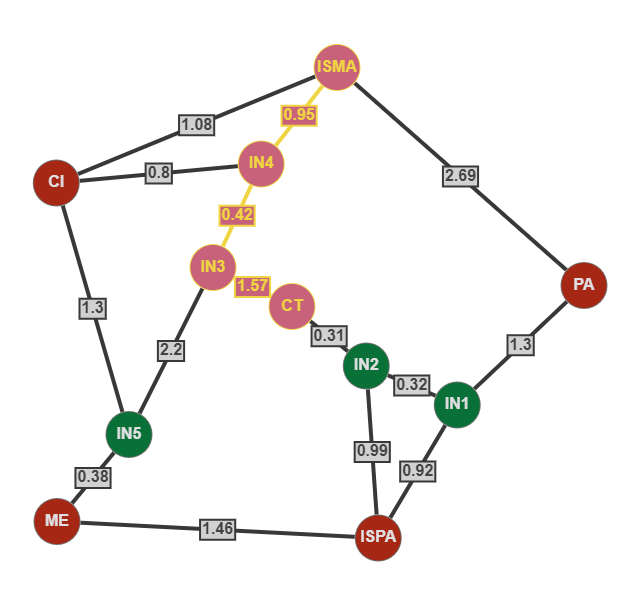
\includegraphics[scale=0.4]{anexos/CT-ISMA.png} &
      \begin{itemize}
        \item Percurso: CT $\rightarrow$ IN3 $\rightarrow$ IN4 $\rightarrow$ ISMA
        \item Custo final: 2,94
      \end{itemize}
    \end{tabular}
    
    \noindent \textbf{Casas do telhado para Centro de Interpretação do românico:}\\
    \begin{tabular}{@{}m{\dimexpr.5\textwidth-.5\columnsep}m{\dimexpr.5\textwidth-.5\columnsep}@{}}
      \centering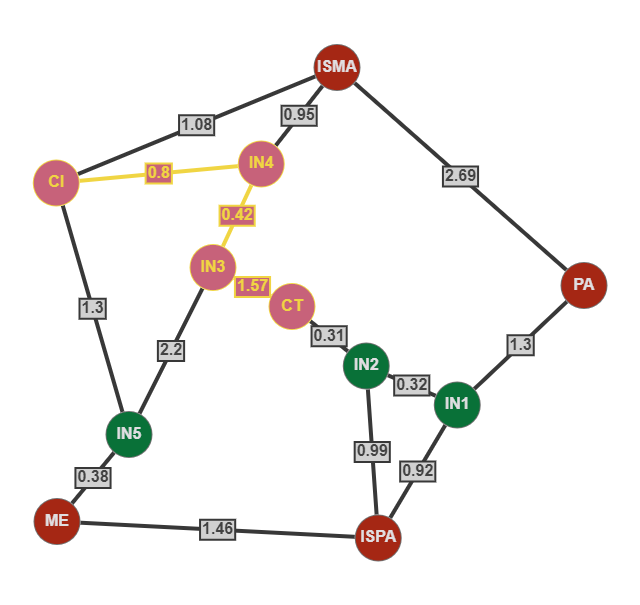
\includegraphics[scale=0.4]{anexos/CT-CI.png} &
      \begin{itemize}
        \item  Percurso: CT $\rightarrow$ IN3 $\rightarrow$ IN4 $\rightarrow$ CI
        \item  Custo final: 2,79
      \end{itemize}
    \end{tabular}

    \noindent \textbf{Casas do telhado para Igreja de São Pedro de Abragão:}\\
    \begin{tabular}{@{}m{\dimexpr.5\textwidth-.5\columnsep}m{\dimexpr.5\textwidth-.5\columnsep}@{}}
      \centering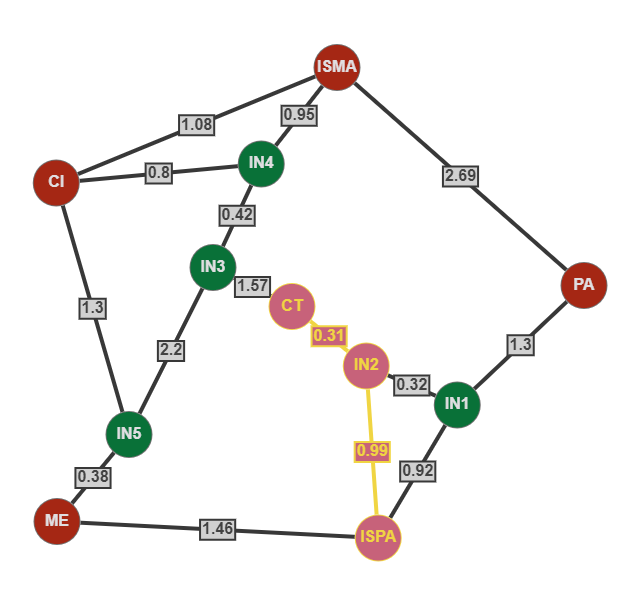
\includegraphics[scale=0.4]{anexos/CT-ISPA.png} &
      \begin{itemize}
        \item Percurso: CT $\rightarrow$ IN2 $\rightarrow$ ISPA
        \item Custo final: 1,3
      \end{itemize}
    \end{tabular}
    
    \newpage
    \noindent \textbf{Ponto do arco para Memorial da Ermida:}\\
    \begin{tabular}{@{}m{\dimexpr.5\textwidth-.5\columnsep}m{\dimexpr.5\textwidth-.5\columnsep}@{}}
      \centering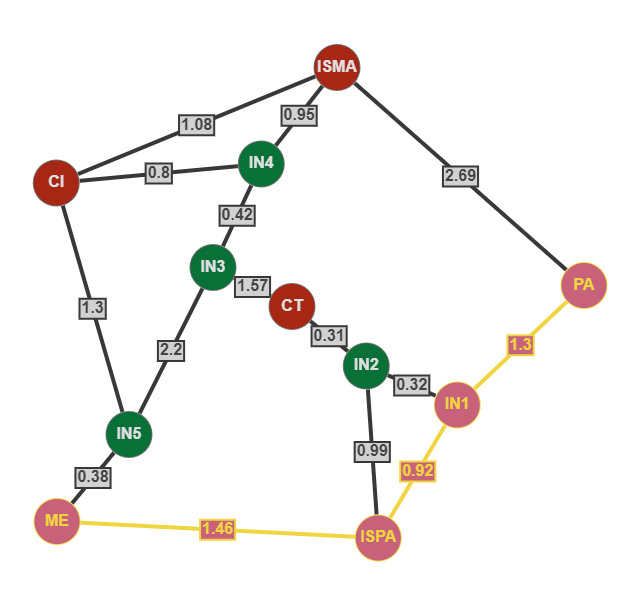
\includegraphics[scale=0.4]{anexos/PA-ME.png} &
      \begin{itemize}
        \item Percurso: PA $\rightarrow$ IN1 $\rightarrow$ ISPA $\rightarrow$ ME
        \item Custo final:3,68
      \end{itemize}
    \end{tabular} 
    
    \noindent \textbf{Ponto do arco para Igreja de Santa Maria de Airães:}\\
    \begin{tabular}{@{}m{\dimexpr.5\textwidth-.5\columnsep}m{\dimexpr.5\textwidth-.5\columnsep}@{}}
      \centering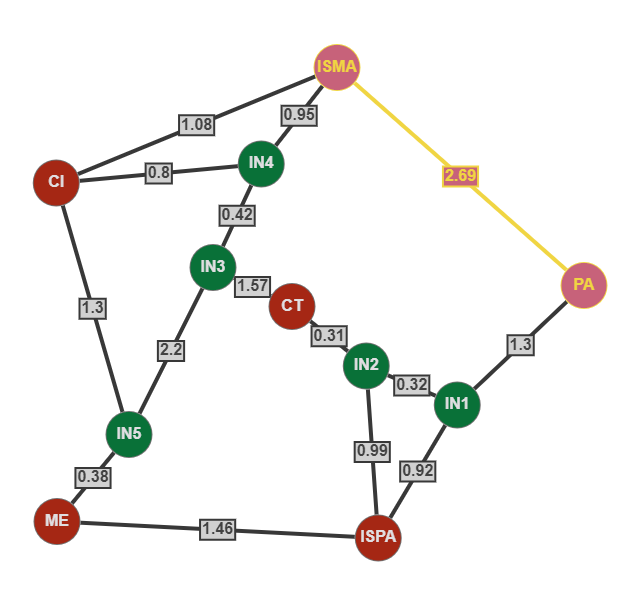
\includegraphics[scale=0.4]{anexos/PA-ISMA.png} &
      \begin{itemize}
        \item Percurso: PA $\rightarrow$ ISMA
        \item Custo final: 2,69
      \end{itemize}
    \end{tabular} 
    
    \noindent \textbf{Ponto do arco para Centro de Interpretação do românico:}\\
    \begin{tabular}{@{}m{\dimexpr.5\textwidth-.5\columnsep}m{\dimexpr.5\textwidth-.5\columnsep}@{}}
      \centering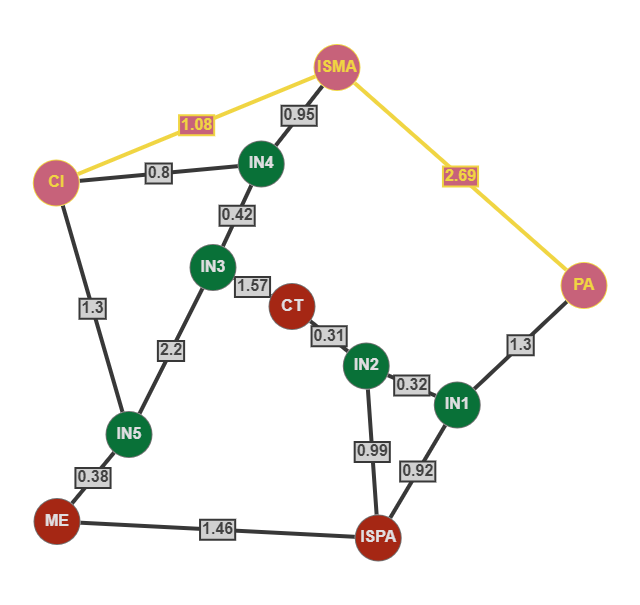
\includegraphics[scale=0.4]{anexos/PA-CI.png} &
      \begin{itemize}
        \item Percurso: PA $\rightarrow$ ISMA $\rightarrow$ CI
        \item Custo final: 3,77
      \end{itemize}
    \end{tabular} 
    
    \newpage
    
    \noindent \textbf{Ponto do arco para Igreja de São Pedro de Abragão:}\\
    \begin{tabular}{@{}m{\dimexpr.5\textwidth-.5\columnsep}m{\dimexpr.5\textwidth-.5\columnsep}@{}}
      \centering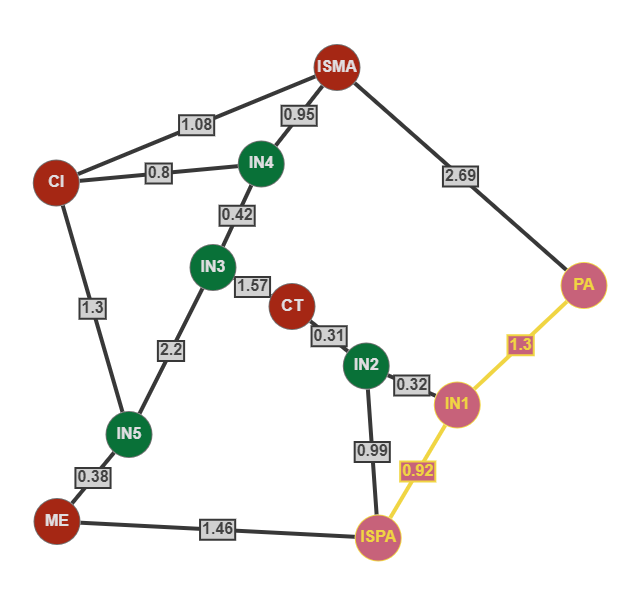
\includegraphics[scale=0.4]{anexos/PA-ISPA.png} &
      \begin{itemize}
        \item Percurso: PA $\rightarrow$ IN1 $\rightarrow$ ISPA
        \item Custo final: 2.22
      \end{itemize}
    \end{tabular} 
    
    \noindent\textbf{ Memorial da Ermida para Igreja de Santa Maria de Airães:}\\
    \begin{tabular}{@{}m{\dimexpr.5\textwidth-.5\columnsep}m{\dimexpr.5\textwidth-.5\columnsep}@{}}
      \centering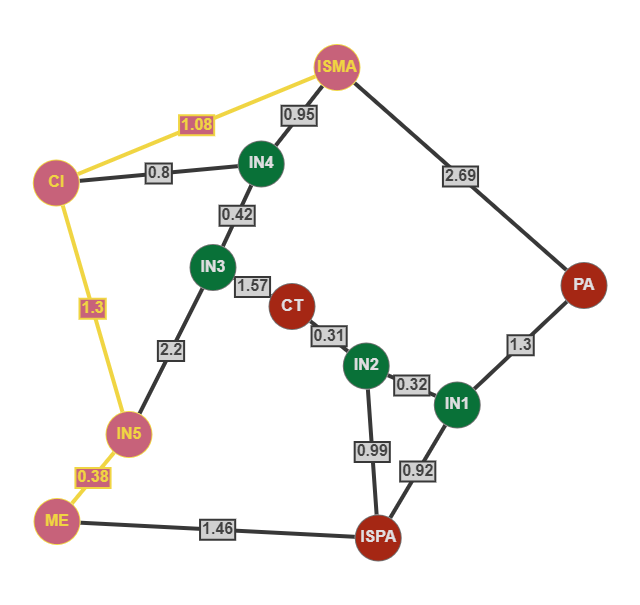
\includegraphics[scale=0.4]{anexos/ME-ISMA.png} &
      \begin{itemize}
        \item Percurso: ME $\rightarrow$ IN5 $\rightarrow$ CI $\rightarrow$ ISMA
        \item Custo final: 2.76
      \end{itemize}
    \end{tabular} 
    
    \noindent \textbf{Memorial da Ermida para Centro de Interpretação do românico:}\\
    \begin{tabular}{@{}m{\dimexpr.5\textwidth-.5\columnsep}m{\dimexpr.5\textwidth-.5\columnsep}@{}}
      \centering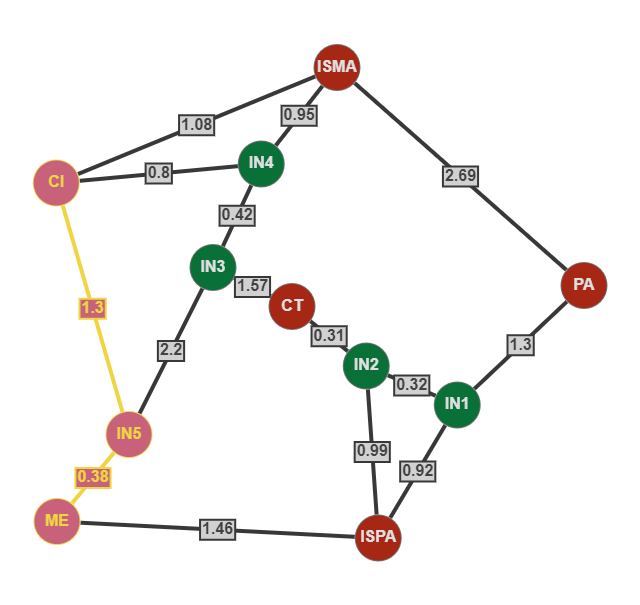
\includegraphics[scale=0.4]{anexos/ME-CI.png} &
      \begin{itemize}
        \item Percurso: ME $\rightarrow$ IN5 $\rightarrow$ CI
        \item Custo final: 1,68
      \end{itemize}
    \end{tabular} 
    
    \newpage
    
    \noindent \textbf{Memorial da Ermida para Igreja de São Pedro de Abragão:}\\
    \begin{tabular}{@{}m{\dimexpr.5\textwidth-.5\columnsep}m{\dimexpr.5\textwidth-.5\columnsep}@{}}
      \centering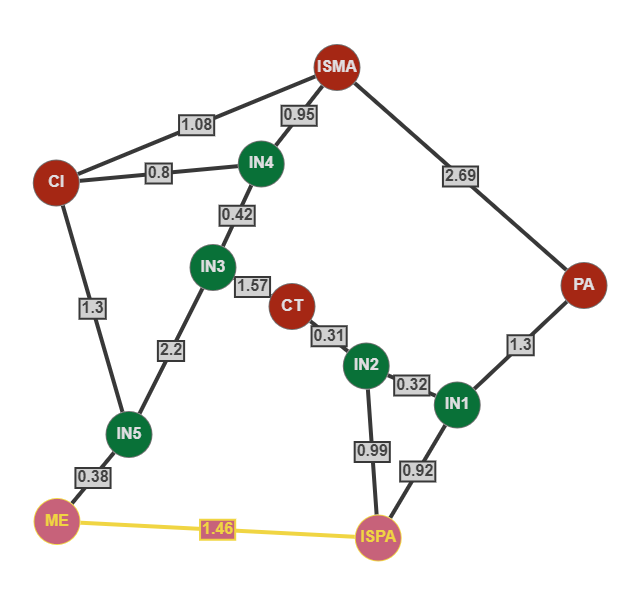
\includegraphics[scale=0.4]{anexos/ME-ISPA.png} &
      \begin{itemize}
        \item Percurso: ME $\rightarrow$ ISPA
        \item Custo final: 1,46
      \end{itemize}
    \end{tabular} 
    
    \noindent \textbf{Igreja de Santa Maria de Airães para Centro de Interpretação do românico:}\\
    \begin{tabular}{@{}m{\dimexpr.5\textwidth-.5\columnsep}m{\dimexpr.5\textwidth-.5\columnsep}@{}}
      \centering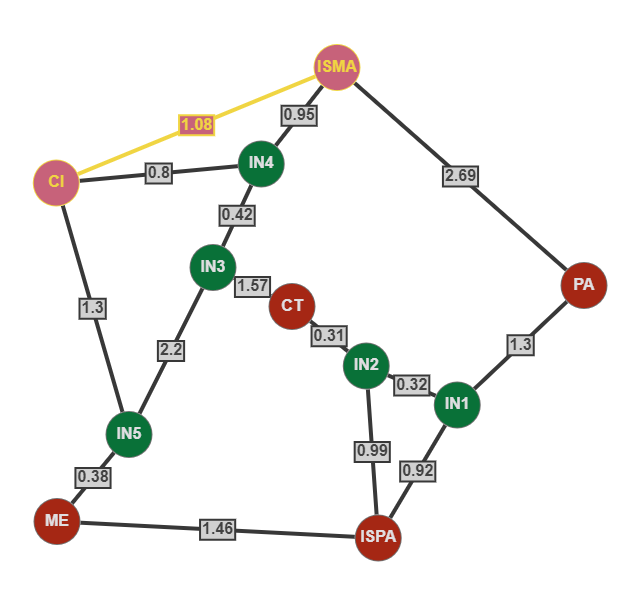
\includegraphics[scale=0.4]{anexos/ISMA-CI.png} &
      \begin{itemize}
        \item Percurso: ISMA $\rightarrow$ CI
        \item Custo final: 1,08
      \end{itemize}
    \end{tabular} 
    
    \noindent \textbf{Igreja de Santa Maria de Airães para Igreja de São Pedro de Abragão:}\\
    \begin{tabular}{@{}m{\dimexpr.5\textwidth-.5\columnsep}m{\dimexpr.5\textwidth-.5\columnsep}@{}}
      \centering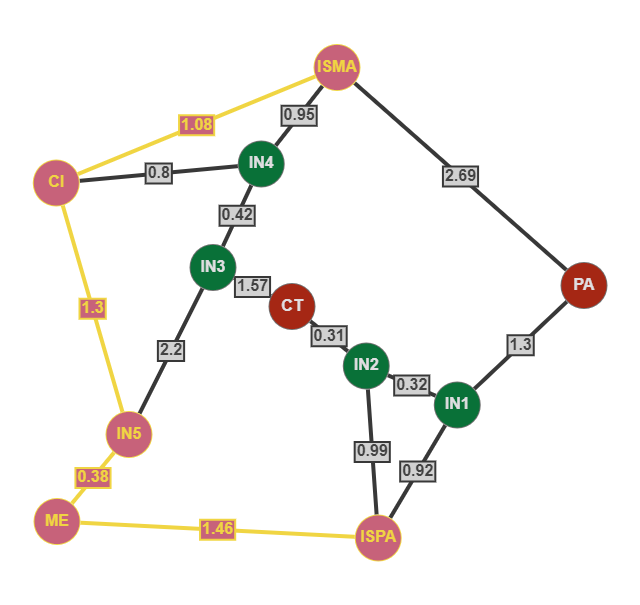
\includegraphics[scale=0.4]{anexos/ISMA-ISPA.png} &
      \begin{itemize}
        \item Percurso: ISMA $\rightarrow$ CI $\rightarrow$ IN5 $\rightarrow$ ME $\rightarrow$ ISPA
        \item Custo final: 4,22
      \end{itemize}
    \end{tabular} 
    
    \newpage
    
    \noindent \textbf{Centro de Interpretação do românico para Igreja de São Pedro de Abragão:}\\
    \begin{tabular}{@{}m{\dimexpr.5\textwidth-.5\columnsep}m{\dimexpr.5\textwidth-.5\columnsep}@{}}
      \centering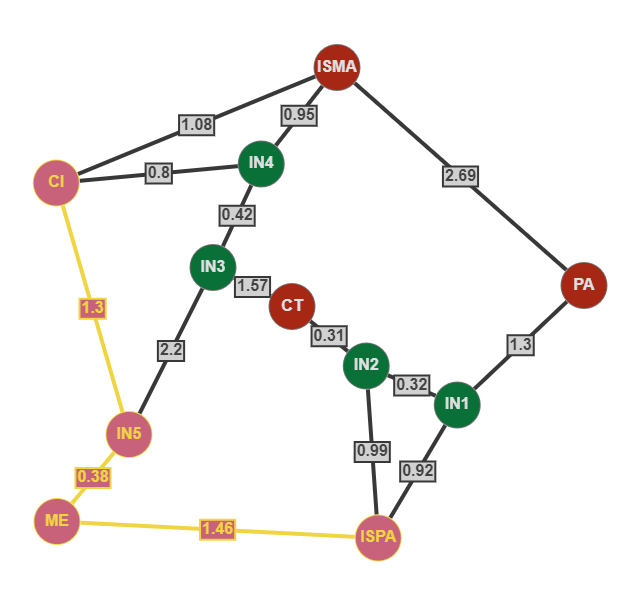
\includegraphics[scale=0.4]{anexos/CI-ISPA.png} &
      \begin{itemize}
        \item Percurso: CI $\rightarrow$ IN5 $\rightarrow$ ME $\rightarrow$ ISPA
        \item Custo final: 3.14
      \end{itemize}
    \end{tabular} 
    
    \begin{center}
        \textbf{Tabela com os custos entre os 5 Monumentos}
    \end{center}
    
    \begin{table}[hbt!]
            \centering
            \begin{tabular}{*{7}{|c}|}
            \hline
            \textbf{Monumentos} & \textbf{CT} & \textbf{ISPA} & \textbf{ME} & \textbf{CI} & \textbf{ISMA} & \textbf{PA}\\ \hline
            \textbf{CT} & 0 & 1.3 & 2.76 & 2.79 & 2.94 & 1.93 \\ \hline
            \textbf{ISPA} & 1.3 & 0 & 1.46 & 3.14 & 4.22 & 2.22 \\ \hline
            \textbf{ME} & 2.76 & 1.46 & 0 & 1.68 & 2.76 & 3.68 \\ \hline
            \textbf{CI} & 2.79 & 3.14 & 1.68 & 0 & 1.08 & 3.77 \\ \hline
            \textbf{ISMA} & 2.94 & 4.22 & 2.76 & 1.08 & 0 & 2.69 \\ \hline
            \textbf{PA} & 1.93 & 2.22 & 3.68 & 3.77 & 2.69 & 0 \\ \hline
        
            \end{tabular}
        \end{table}
    \newpage
     \subsubsection{c) O percurso com menor custo com partida no alojamento e que permita visitar todos os 5 locais uma única vez e regressar ao local de partida)}
     
    \noindent Esta pergunta é muito parecida com o problema do Caixeiro Viajante.
    O problema do Caixeiro Viajante consiste em dado um conjunto de cidades e a distância entre cada par de cidades, encontrar a rota mais curta possível que visite todas as cidades exatamente uma única vez e retorne ao ponto de partida.\\
    Para resolver o problema do Caixeiro Viajante existem diversos algoritmos como:
\begin{itemize}
\item Algoritmo força bruta que consiste em gerar as várias soluções possíveis e verificar a que satisfaz a condição do problema (percurso com menor custo).
\item Algoritmo Branch and bound que consiste em subdividir o problema  em problemas mais pequenos, de forma a obter a melhor solução.
\item Algoritmo do Vizinho Mais Próximo que consiste em escolher um ponto de partida e de entre as arestas adjacentes escolher a que tem menor peso partindo para esse vértice a que chamamos vizinho mais próximo.
\end{itemize} 
    
    \noindent Para a resolução desta alínea utilizamos o algoritmo da força bruta pois é um dos mais fáceis de aplicar, apesar de não ser um dos mais eficientes é um dos mais exatos pois funciona como "tentativa e erro", tornando-se assim bastante preciso visto que a probabilidade de não obter o melhor caminho é muito ínfima.

    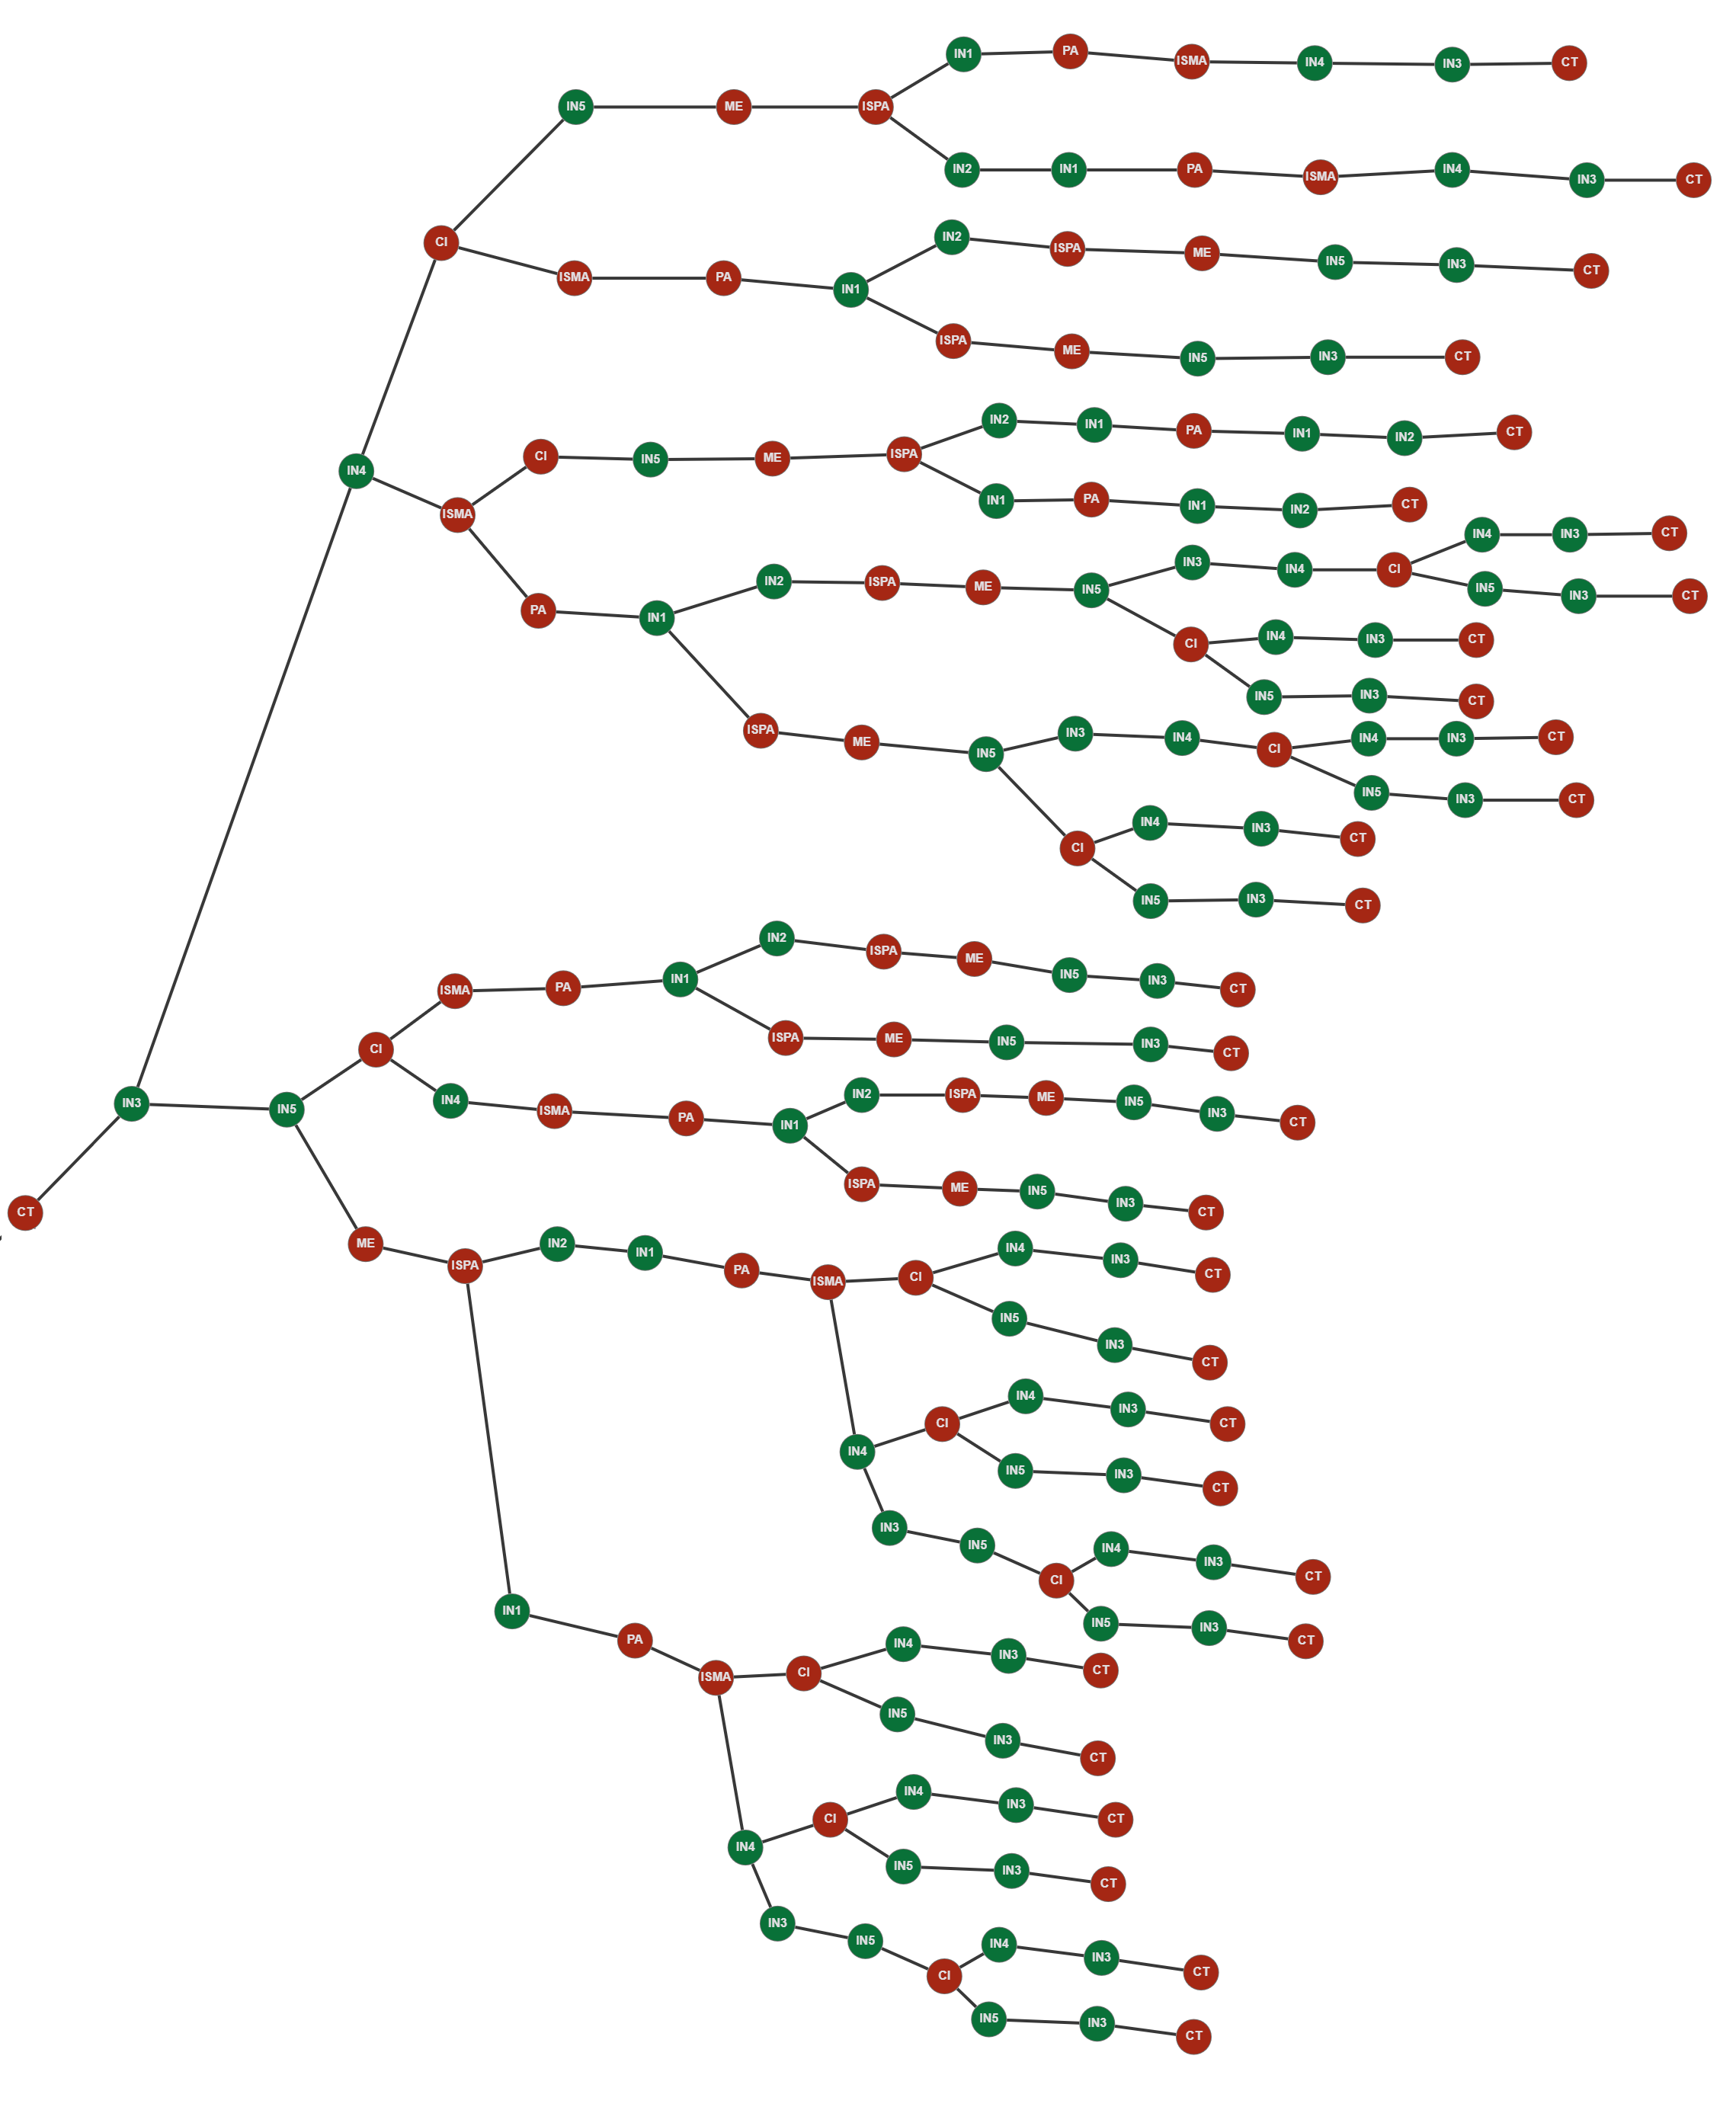
\includegraphics[scale=0.25]{anexos/ArvoreFinal2.png}
    \newpage
    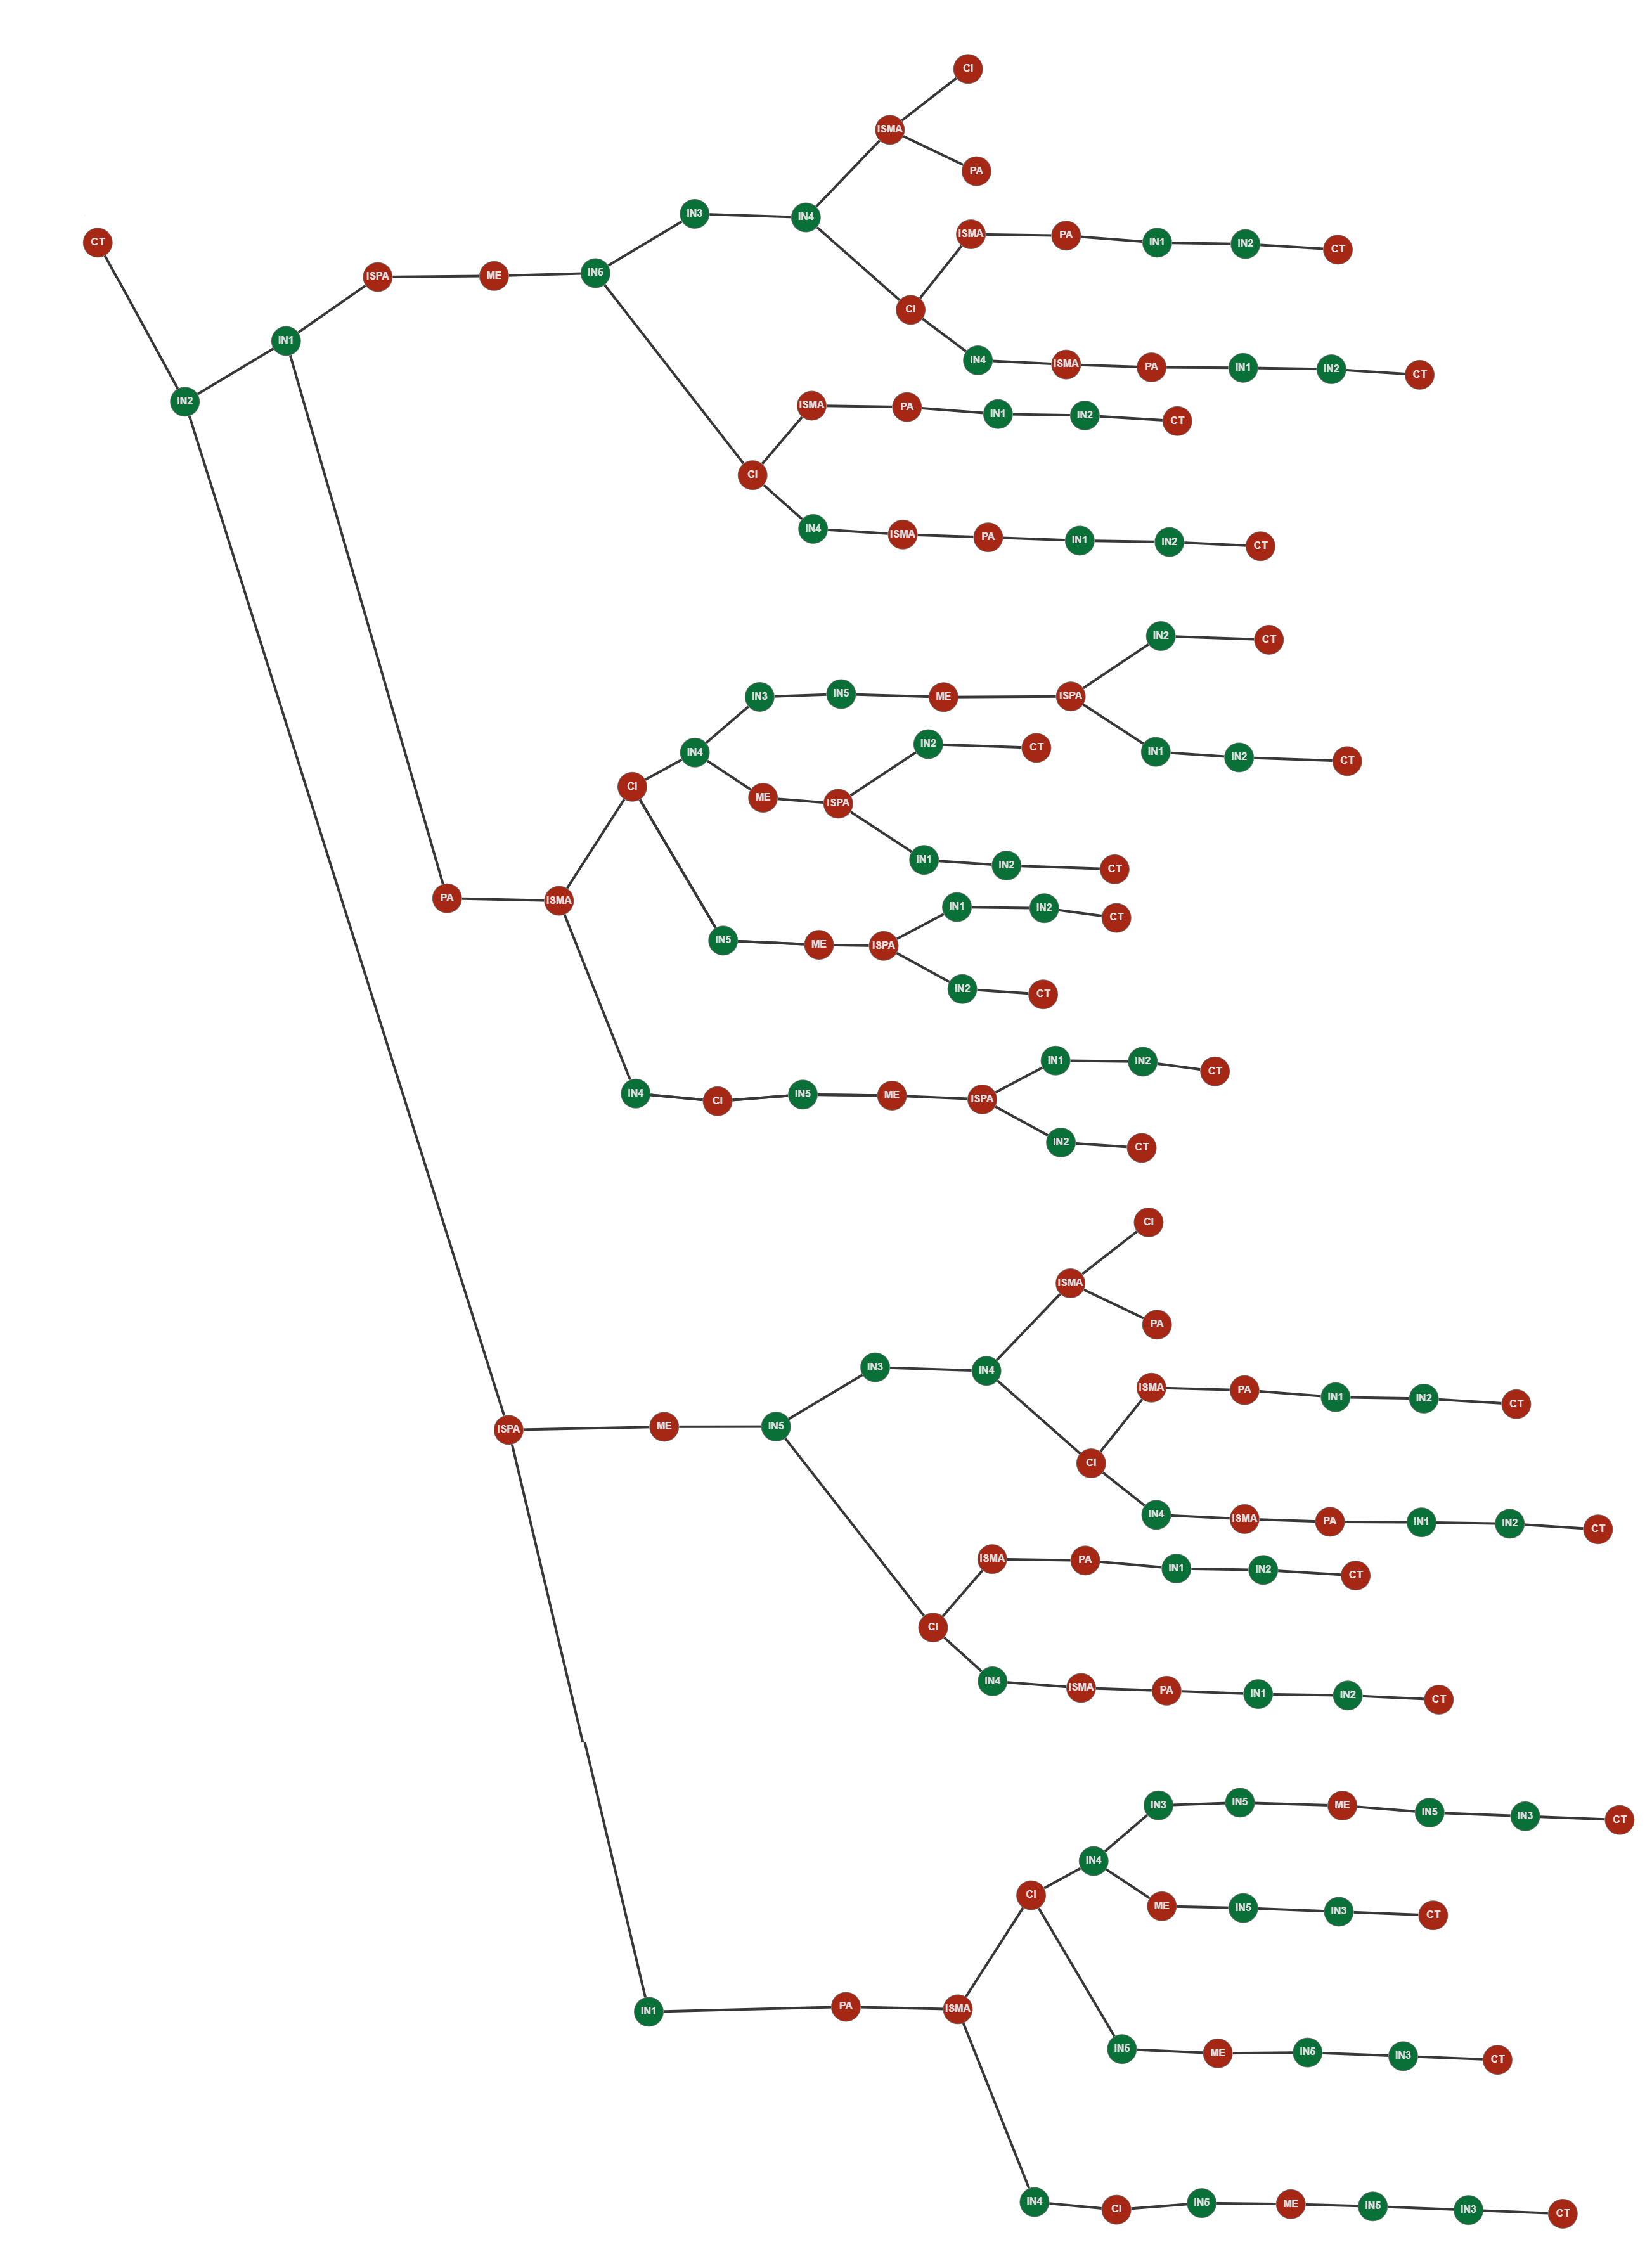
\includegraphics[scale=0.23]{anexos/ArvoreFinal1.png}
    \newpage    
    \noindent\textbf{ Parte dos cálculos}\\\\
    CT IN3 IN4 CI IN5 ME ISPA IN1 PA ISMA IN4 IN3 CT = 14,73\\
    CT IN3 IN4 CI IN5 ME ISPA IN2 IN1 PA ISMA IN4 IN3 CT = 14,58\\
    CT IN3 IN4 CI ISMA PA IN1 IN2 ISPA ME IN5 IN3 CT = 16,08\\
    CT IN2 ISPA ME IN5 IN3 IN4 CI ISMA PA IN1 IN2 CT = 12.26\\
    CT IN2 ISPA ME IN5 CI ISMA PA IN1 IN2 CT = 8.78\\
    CT IN3 IN5 CI ISMA PA IN1 IN2 ISPA ME IN5 IN3 CT = 17,06\\
    CT IN3 IN5 CI ISMA PA IN1 ISPA ME IN5 IN3 CT = 16,67\\
    CT IN2 IN1 ISPA ME IN5 IN3 IN4 CI ISMA PA IN1 IN2 CT = 12.51\\
    CT IN2 IN1 ISPA ME IN5 IN3 IN4 CI IN4 ISMA PA IN1 IN2 CT = 13.18\\
    CT IN2 IN1 ISPA ME IN5 CI ISMA PA IN1 IN2 CT = 10.39\\
    CT IN2 IN1 ISPA ME IN5 CI IN4 ISMA PA IN1 IN2 CT = 11.06\\
    CT IN2 IN1 PA ISMA CI IN4 IN3 IN5 ME ISPA IN2 CT = 12.26
    \begin{center}
         \textbf{...}
    \end{center}
    \noindent \textbf{Caminho mais curto}:  CT IN2 ISPA ME IN5 CI ISMA PA IN1 IN2 CT\\
    \noindent \textbf{Custo do caminho mais curto}: 8.78
    
    \newpage
    \subsection{3. Exercício de Criptografía}
    
    \begin{table}[hbt!]
        \scalebox{0.7}{
        \begin{tabular}{*{29}{|c}|}
            \hline
            A & B & C & D & E & F & G & H & I & J & K  & L  & M  & N  & O  & P  & Q  & R  & S  & T  & U  & V  & W  & X  & Y  & Z  & .  & ,  & !  \\ \hline
            0 & 1 & 2 & 3 & 4 & 5 & 6 & 7 & 8 & 9 & 10 & 11 & 12 & 13 & 14 & 15 & 16 & 17 & 18 & 19 & 20 & 21 & 22 & 23 & 24 & 25 & 26 & 27 & 28 \\ \hline
        \end{tabular}}
    \end{table}
    
    \subsubsection{3.1. Encriptação }
    \noindent \textbf{Nesta questão é pedido para encriptar a mensagem "Venha experimentar, saborear e sentir. . . Felgueiras!” que é o slogan do Turismo de Felgueiras (https://visitfelgueiras.com/), acrescentando, "é o conselho de ... 4 primeiros nomes de cada um dos estudantes do grupo" através da seguinte função:  \(f(p) = (\beta p+ 2) \mod 29\), onde \(\beta \neq 0\) e é o último algarismo do número de aluno de um dos elementos do grupo.}\\
    
    \noindent Para \(\beta\) decidimos que seria \(\beta=6\), que vem do número mecanográfico 8200586, então:
    \begin{center}
    \(f(p) = (\beta p+ 2) \mod 29 = (6 p+ 2) \mod 29\)\\
    \end{center}
    
    \noindent Calculo auxiliar verificar se a função é bijetiva:\\
    \noindent Para isso o mdc(6, 29) tem de ser igual a 1, ou seja, são primos entre si.\\
    O máximo divisor comum são todos os fatores comuns elevados ao menor expoente.
    \begin{center}
    \begin{tabular}[hbt!]{c|c}
    6 & 2\\
    3 & 3\\
    1 & 
    \end{tabular} \hspace{1cm}
    \begin{tabular}[hbt!]{c|c}
    29 & 29\\
    1 &
    \end{tabular}
    \end{center}
    
    \noindent Após obtermos a função de encriptação, já podemos encriptar a frase. Para isso temos de ir à tabela e ver a que número corresponde cada letra da frase e substituir o \(p\) na função \(f(p)\).\\
    
     \noindent Frase original: Venha experimentar, saborear e sentir... Felgueiras! e o conselho de Bruno, Goncalo, Jorge e Nuno
     
         
    \begin{center}
    \begin{tabular}{@{}l@{}}
    \(V = 21 \rightarrow f(21) = (6 \times 21 + 2) \mod 29 = 12 \rightarrow M \)\\
     \(e = 4 \rightarrow f(4) = (6 \times 4 + 2) \mod 29 = 26 \rightarrow . \)\\
     \(n = 13 \rightarrow f(13) = (6 \times 13 + 2) \mod 29 = 22 \rightarrow W \)\\
     \(h = 7 \rightarrow f(7) = (6 \times 7 + 2) \mod 29 = 15 \rightarrow P \)\\
     \(a = 0 \rightarrow f(0) = (6 \times 0 + 2) \mod 29 = 2  \rightarrow C \)\\
    \end{tabular}
    \end{center}
    
    \noindent Para tornar este processo mais rápido decidimos criar um programa em python para efetuar a encriptação da frase que queremos encriptar.\\
    \newpage
    \noindent Este programa recebe uma frase, o número a ser multiplicado e o a ser somado, de seguida são efetuados os respetivos cálculos para cada caracter e após encriptar todos os carateres, é retornada a frase encriptada para o utilizador. Para verificar se é possível encriptar utilizamos um algoritmo já existente que se encontra no seguinte link \url{https://www.rookieslab.com/posts/extended-euclid-algorithm-to-find-gcd-bezouts-coefficients-python-cpp-code}.\\\\
    Exemplo execução:
    \begin{center}
        \fbox{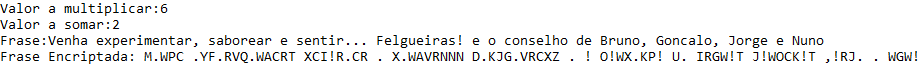
\includegraphics[scale=0.65]{anexos/encripta.png}}
    \end{center}
    
    \noindent Tabela de encriptação:\\
    \begin{table}[hbt!]
        \scalebox{0.605}{
        \begin{tabular}{*{30}{|c}|}
            \hline
             Original & A & B & C & D & E & F & G & H & I & J & K  & L  & M  & N  & O  & P  & Q  & R  & S  & T  & U  & V  & W  & X  & Y  & Z  & .  & ,  & !  \\ \hline
             \(p\) & 0 & 1 & 2 & 3 & 4 & 5 & 6 & 7 & 8 & 9 & 10 & 11 & 12 & 13 & 14 & 15 & 16 & 17 & 18 & 19 & 20 & 21 & 22 & 23 & 24 & 25 & 26 & 27 & 28 \\ \hline
            \(f(p)\) & 2 & 8 & 14 & 20 & 26 & 3 & 9 & 15 & 21 & 27 & 4 & 10 & 16 & 22 & 28 & 5 & 11 & 17 & 23 & 0 & 6 & 12 & 18 & 24 & 1 & 7 & 13 & 19 & 25 \\ \hline
           Criptografada & C & I & O & U & . & D & J & P & V & , & E & K & Q & W & ! & F & L & R & X & A & G & M & S & Y & B & H & N & T & Z \\ \hline
        \end{tabular}}
    \end{table}
    
    \noindent Frase original: Venha experimentar, saborear e sentir... Felgueiras! e o conselho de Bruno, Goncalo, Jorge e Nuno\\
    
    \noindent Frase Criptografada: M.WPC .YF.RVQ.WACRT XCI!R.CR . X.WAVRNNN D.KJG.VRCXZ . ! O!WX.KP! U. IRGW!T J!WOCK!T ,!RJ. . WGW!
    
    \newpage
    \subsubsection{3.2. Desencriptação}
    \noindent \textbf{Nesta questão é pedido para desencripte a mensagem obtida na alínea anterior.}\\
    \noindent A partir da função  \(f(p) = (6 p+ 2) \mod 29\), que foi obtida na alínea anterior será feita a desencriptação.\newline
    
    \noindent Para fazer a desencriptação temos de encontrar uma expressão para \( f^{-1}(x)\)
    \begin{center}
    \begin{tabular}{@{}l@{}}
        $(6 p + 2) \mod29 = y$\\
        $(6 p)\mod29 + 2\mod 29= y$\\
        $(6 p)\mod29 = y - 2$\\
        $6 p \equiv (y - 2) \mod29$
    \end{tabular}
    \end{center}
   \noindent  Calculo auxiliar do inverso de \( 6\mod29\) :\\\\
    \noindent Antes de calcular o inverso temos de verificar se é possível.\\
    \noindent Para isso mdc(6, 19)=1 e como já visto em cima é verdade, assim sendo a função é invertível.\\\\
    Agora temos de aplicar o algoritmo de Euclides para obtermos os coeficientes de Bézout:
    \begin{center}
    \begin{tabular}{@{}l@{}}
        $a\times6\equiv1\mod29$\\\\
        $29 = 6\times4 + 5 \rightarrow 5 = 29 - 6 \times 4$\\
        $6 = 5\times1 +1 \hspace*{1.9mm} \rightarrow 1 = 6 - 5 \times 1$\\
        \hspace*{3.6cm}$= 6 - (29 - 6 \times 4) \times 1$\\
        \hspace*{3.6cm}$= 6 - 29 \times 1 + 6 \times 4$\\
        \hspace*{3.6cm}$= -29 \times 1 + 6 \times 5$\\
    \end{tabular}
    \end{center}
    
    \noindent Por fim descobrimos que os coeficientes de Bézout são 1 e 5.
    
    \vspace{0.5cm}
    \noindent Agora temos de multiplicar a função pelo coeficientes de Bézout do número 6 que é 5.
    \begin{center}
        \noindent \begin{tikzcd}
            6 p \equiv (y - 2) \mod29 \arrow[black, bend right]{rr}[black,swap]{\times5} & (=) & \cancel{5\times6}p \equiv (5y - 10) \mod29
        \end{tikzcd}
    \end{center}
    
    \newpage
    \noindent Então a função da desencriptação é:
    \begin{center}
    \noindent \(f^{-1}(y) = (5y - 10) \mod29 = (5y + 19) \mod29\)
    \end{center}
    
    \noindent Cálculo Auxiliar:\\
    Como 29 divide \(19 - (-10) = 29\), temos que \(19 \equiv -10 \mod29\).
    
    \noindent
    
    \begin{center}
    \begin{tabular}{@{}l@{}}
    \(M = 12 \rightarrow f(12) = (5 \times 12 + 19) \mod 29 = 21 \rightarrow V \)\\
    \(. = 26 \rightarrow f(26) = (5 \times 26 + 19) \mod 29 = 4 \rightarrow E \)\\
    \(W = 22 \rightarrow f(22) = (5 \times 22 + 19) \mod 29 = 13 \rightarrow N \)\\
    \(P = 15 \rightarrow f(15) = (5 \times 15 + 19) \mod 29 = 7 \rightarrow H \)\\
    \(C = 2 \rightarrow f(2) = (5 \times 2 + 19) \mod 29 = 0 \rightarrow A \)\\
    \end{tabular}
    \end{center}
    \noindent Para tornar este processo mais rápido decidimos usar o programa da encriptação, usando os dados da função \(f^{-1}(y)\).\\\\
    Exemplo execução:
    \begin{center}
        \fbox{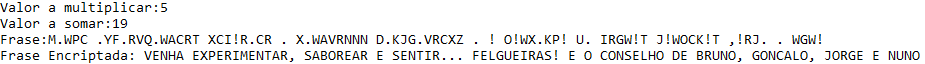
\includegraphics[scale=0.65]{anexos/encripta1.png}}
    \end{center}
    
    \noindent Tabela de desencriptação:
    \begin{table}[hbt!]
        \scalebox{0.605}{
        \begin{tabular}{*{30}{|c}|}
            \hline
            Criptografada & C & I & O & U & . & D & J & P & V & , & E & K & Q & W & ! & F & L & R & X & A & G & M & S & Y & B & H & N & T & Z \\ \hline
            \(y\) & 2 & 8 & 14 & 20 & 26 & 3 & 9 & 15 & 21 & 27 & 4 & 10 & 16 & 22 & 28 & 5 & 11 & 17 & 23 & 0 & 6 & 12 & 18 & 24 & 1 & 7 & 13 & 19 & 25 \\ \hline
            \(f^{-1}(y)\) & 0 & 1 & 2 & 3 & 4 & 5 & 6 & 7 & 8 & 9 & 10 & 11 & 12 & 13 & 14 & 15 & 16 & 17 & 18 & 19 & 20 & 21 & 22 & 23 & 24 & 25 & 26 & 27 & 28 \\ \hline
            Original & A & B & C & D & E & F & G & H & I & J & K  & L  & M  & N  & O  & P  & Q  & R  & S  & T  & U  & V  & W  & X  & Y  & Z  & .  & ,  & !  \\ \hline
        \end{tabular}}
    \end{table}\\
    \noindent Frase criptografada: M.WPC .YF.RVQ.WACRT XCI!R.CR . X.WAVRNNN D.KJG.VRCXZ . ! O!WX.KP! U. IRGW!T J!WOCK!T ,!RJ. . WGW!\\
    
    \noindent Frase descriptografada: VENHA EXPERIMENTAR, SABOREAR E SENTIR... FELGUEIRAS! E O CONSELHO DE BRUNO, GONCALO, JORGE E NUNO\\
   
    \noindent Para tornar o processo da desencriptação mais fácil e rápido decidimos criar um programa em python.\\\\
    \noindent Este programa recebe uma frase encriptada, o número a ser multiplicado e o a ser somado na encriptação, e de seguida são efetua os respetivos cálculos para cada carater e após encriptar todos os carateres, é retornada a frase desencriptada para o utilizador.
    Para descobrir os coeficientes de Bézout e o mdc utilizamos um algoritmo já existente que se encontra no seguinte link \url{https://www.rookieslab.com/posts/extended-euclid-algorithm-to-find-gcd-bezouts-coefficients-python-cpp-code}\\\\
    Exemplo execução:
    \begin{center}
        \fbox{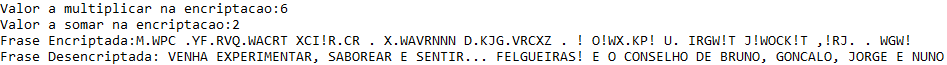
\includegraphics[scale=0.6]{anexos/desencriptada.png}}
    \end{center}
     \newpage
    
    \section{Conclusão}
    \noindent Ao longo deste trabalho surgiram algumas dúvidas que foram esclarecidas pelas professoras responsáveis da Unidade Curricular e através de algumas pesquisas na Internet. Na nossa opinião achamos que o trabalho foi concluído com sucesso sendo que solucionamos todos os exercícios com sucesso explicando sempre as nossas resoluções e apresentando sempre outras possíveis soluções.\\
    
    \noindent Tal como já foi referido na introdução deste relatório, todos os conceitos abordados serão bastante importantes para o nosso futuro sendo que temos vários exemplos em que estes conhecimentos podem ser utilizados, como por exemplo:\\
    
    \noindent \textbf{Exemplo do uso da recursividade}:\\
    A recursividade é bastante utilizada na programação quando uma parte do algoritmo necessita do resultado da última iteração, este processo permite obter uma maior legibilidade do código bem como uma melhoria em termos de processamento.\\
    
    \noindent\textbf{Exemplo de uso da Teoria de Grafos:}\\
    Temos como exemplo uma estrutura de ligação de um Website de artigos onde os vértices podem ser os artigos em questão e as arestas as ligações entre os diversos artigos, ou seja, imaginando que temos o artigo A e o artigo B se existir uma aresta entre estes dois vértices significa que existe por exemplo um link do artigo A para o B.\\
    
    \noindent\textbf{Exemplo de encriptação e desencriptação:}\\
    A encriptação e desencriptação são conceitos muito importantes sendo que, num contexto empresarial, existe sempre informação confidencial que tem de ser protegida e, para isso é então utilizada a encriptação para que esta informação não seja visualizada por qualquer um e apenas por pessoas que tenham acesso ao algoritmo de desencriptação.\\

    \noindent Concluímos assim que este trabalho além de ser útil para demonstrarmos os nossos conhecimentos, foi também muito importante para a aprendizagem de novos conceitos relacionados com a matéria.


    \newpage
    
    \section{Bibliografia}
    \nocite{ euclid, grafos, inducao, EGV, scilab, graphtea, overleaf, rota, tablesgenerator, waze, dijkstra}
    \printbibliography[heading=none]


\end{document}